\subsection{Introducción}

En la siguiente etapa del informe, se presenta el desafío de analizar, confeccionar y evaluar un controlador de tonos. Para ello, primero se decidió observar el funcionamiento del oído humano, ya que de esta forma se logra comprender un poco más como se interpretan las diversas frecuencias por el sistema auditivo, para luego entrar en lo que a la electrónica respecta.

\subsection{Fisiología del oído}

%La fisiología auditiva se encuentra dada en tres estructuras:
%\begin{itemize}
%	\item Oído externo:
%	Este conforma parte del órgano periférico encargado de la conducción de estímulos externos, transmitiendolos hacia el canal auditivo externo. Las paredes rígidas de este último evitan que el sonido sea absorbido por por los demás tejidos blandos.
%	\item Oído medio:
%	Compuesto por el sistema timpanoosicular (membrana timpánica y los tres huesillos: martillo, yunque y estribo), cumple con la función tanto de transmitir las señales del ambiente, como de proteger las estructuras neurosensoriales del oído interno y de la ventana redonda.
%	\item Oído interno:
%	Constituido por el laberinto óseo y dentro de este, el membranoso. Comprende dos aparatos desde el punto de vista anatómico y funcional: el coclear, encargado de la audición y por ende, del desarrollo del lenguaje, y el vestibular, que es el órgano que se ocupa del equilibrio\footnote{Diamante, V. (2004). Otorrinolaringología y afecciones conexas. Buenos Aires: El Ateneo.}.
%\end{itemize}

Cualquier señal captada por el odio humano se caracteriza por poseer una amplitud variable, la cual crece hasta alcanzar un máximo, para luego decrecer abruptamente. Además, dependiendo de la frecuencia de dicha onda, varía el sitio de la cóclea donde se presenta la máxima amplitud. De esta forma, el pico de amplitud se presenta en las inmediaciones del vértice de la cóclea para las frecuencias bajas (graves), mientras que para las altas (agudas), en la vecindad del vestíbulo\footnote{Diamante, V. (2004). Otorrinolaringología y afecciones conexas. Buenos Aires: El Ateneo.}.

\begin{figure}[H]
\centering
	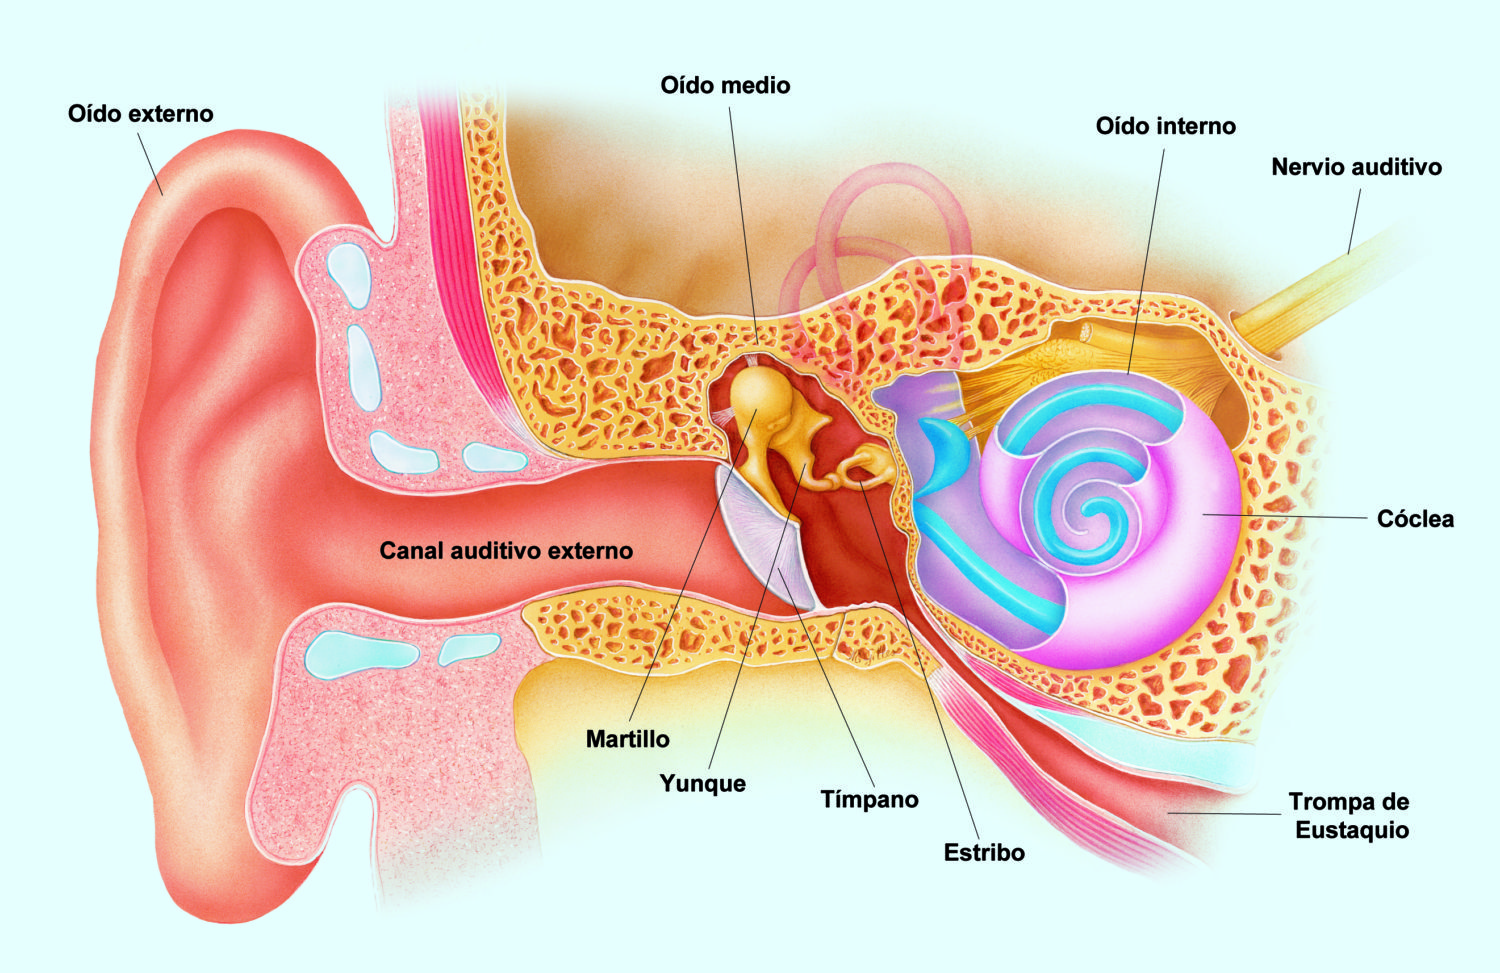
\includegraphics[width=0.6\textwidth]{Imagenes/Partes-del-oido.png}
	\caption{Estructura interna del oído.}
	\label{fig:oido}
\end{figure}

El ser humano puede detectar frecuencias entre los $20 \ Hz$ y los $20 \ kHz$.\footnote{En.wikipedia.org. (2019). Audio frequency. [online] Available at: \url{https://en.wikipedia.org/wiki/Audio_frequency} [Accessed 11 Sep. 2019].} A continuación, se realiza un detenimiento en el análisis de la ganancia del oído medio y externo. Es así que se muestra en la Figura (\ref{fig:oidoganancia}) la ganancia del oído externo, medio y la suma de ambas. Se destaca como las frecuencias menores a $1500 \ Hz$ no son prácticamente alteradas por el oído externo, mientras que la ganancia del oído medio se asemeja a un filtro pasa-banda al rededor de $1 \ kHz$. Finalmente, se puede decir que la suma de ambas converge en un gran filtro pasa-banda, cuyo pico máximo se encuentra cercano a los $3 \ kHz$. Es importante esta observación, ya que dicho filtro es el que determina el espectro audible por el ser humano.\footnote{S. Rosen and P. Howell, Signals and systems for speech and hearing, 2nd ed. 2011.}
\begin{figure}[H]
\centering
	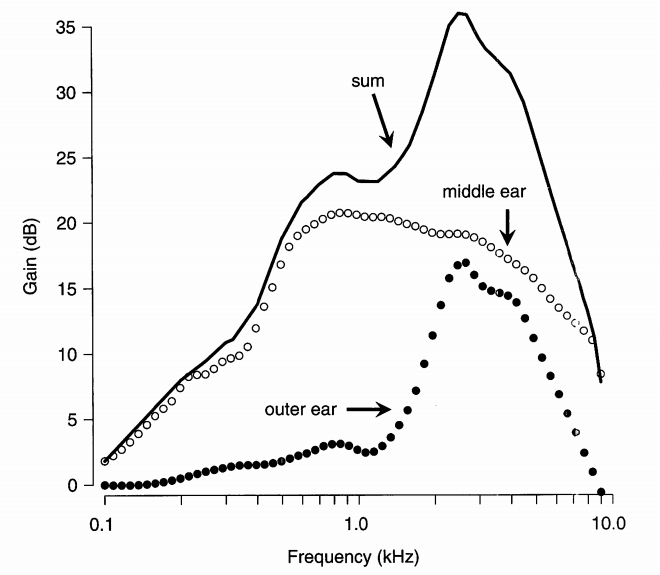
\includegraphics[width=0.5\textwidth]{Imagenes/Ganancia-del-oido-externo-y-medio.png}
	\caption{Ganancia del oído externo, medio y total.}
	\label{fig:oidoganancia}
\end{figure}

Es así que se presenta una división de las bandas de frecuencia audibles por el oído humano\footnote{``Ecualización Básica: Todo lo que necesitas saber sobre la Ecualización | LANDR Blog'', LANDR Blog, 2019. [Online]. Available: \url{https://blog.landr.com/es/ecualizacion-basica-todo-lo-que-necesitas-saber-sobre-la-ecualizacion/}. [Accessed: 11- Sep- 2019].}.
\begin{figure}[H]
\centering
	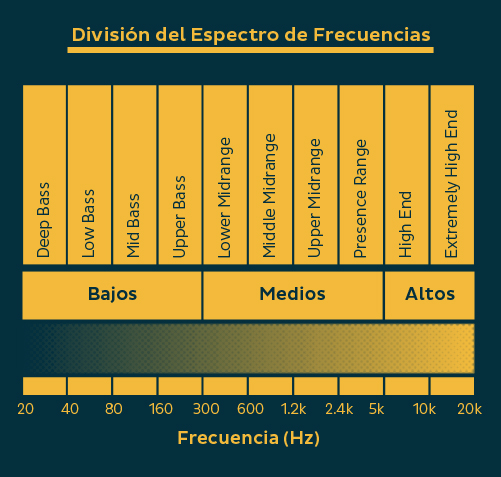
\includegraphics[width=0.5\textwidth]{Imagenes/FrequencySpectrumDivision.png}
	\caption{División del espectro de frecuencias audibles.}
	\label{fig:divfreq}
\end{figure}

A partir de aquí, se considera los rangos de frecuencias bajas, medias y altas a las presentadas en la Figura (\ref{fig:divfreq}).
%Cabe destacar que las señales existentes en el ambiente pueden ser detectadas de dos formas distintas: mediante la vía aérea, es decir, a través el mecanismo explicado previamente, y mediante vibraciones óseas del cráneo. Mientras que el umbral de adución de la primera es teóricamente de $0 \ dB$, la segunda posee un umbral mínimo de $60 \ dB$. 

%Para finalizar esta sección, se define cuando una persona sufre de una perdida de audición. Esta se da un individuo no puede oír o posee un umbral de audición mayor o igual a 25 dB. Para alcanzar esto, se debe superar el nivel máximo de exposición sin riesgos, el cual es de $85 \ dB$ durante 8 horas.\footnote{``Escuchar sin riesgos!'', Who.int, 2019. [Online]. Available: \url{https://www.who.int/pbd/deafness/activities/MLS_Brochure_Spanish_lowres_for_web.pdf}. [Accessed: 11- Sep- 2019].}

\subsection{Funcionamiento de un ecualizador}

Un equalizador es un dispositivo que se caracteriza por modificar la amplitud de los coeficientes de Fourier de una señal. En otras palabras, permite modificar la ganancia de las frecuencias bajas, medias y altas de una señal. Para ello, se basa en la combinación de distintos filtros pasa-banda, con amplificación variable, cuya combinación permite dar con la configuración deseada.

Existen distintos tipos de ecualizadores, con mayores y menores grados de libertad sobre las bandas, es decir, filtros selectores que amplifican o atenúan ciertas bandas de frecuencias. En el presente informe se desarrolló un filtro de tres bandas. Para poder concebir dicho dispositivo, primero se analizó el circuito mostrado en la Figura (\ref{fig:circuitoini}).

\begin{figure}[H]
\begin{center}
\begin{circuitikz}
	\node [op amp](A){};
	\draw (A.+) to[short] ++(-0.5,0) to[short] ++(0,-1) node[ground]{};
	\draw (A.-) to[short] ++(-0.5,0) to[short] ++(0,1.5) node[](v1){} to[R, l = $R_3$] ++(-3.5,0) to[short] ++(0,3);
	\draw (v1) to[R, l_= $R_3$] ++(3.5,0) to[short] ++(0,3);
	\draw (v1) to[open] ++(0,3) node[potentiometershape, rotate=180, label=south:$R_2$](P){};
	\draw (v1) to[C, l = $C_2$] (P.wiper);
	\draw (P.right) to[R, l= $R_1$] ++(-4,0) node[ocirc,label=left:$V_{in}$]{};
	\draw (P.left) to[R, l_= $R_1$] ++(4,0) node[ocirc,label=right:$V_{out}$]{};
	\draw (P.right) to[open] ++(-0.5,0) to[short] ++(0,1.5) to[C, l = $C_1$] ++(2.2,0) to[short] ++(0,-1.5);
	\draw (A.out) to[short] ++(0.62,0) to[short] ++(0,2);
\end{circuitikz}
	\caption{Circuito analizado.}
	\label{fig:circuitoini}
\end{center}
\end{figure}

Para facilitar el análisis, se reemplaza el potenciómetro $R_2$ con dos resistencias fijas, tal que se cumpla $R_2 = R_{2}^{'} + R_{2}^{''} $, considerando que
\begin{equation}
\begin{split}
	R_{2}^{'} &= \psi R_2\\ R_{2}^{''} &= \left( 1 - \psi \right) R_2
\end{split}
\label{equ:r2p}
\end{equation}
siendo $0 \leq \psi \leq 1$.

\begin{figure}[H]
\begin{center}
\begin{circuitikz}
	\node [op amp](A){};
	\draw (A.+) to[short] ++(-0.5,0) to[short] ++(0,-1) node[ground]{};
	\draw (A.-) to[short] ++(-0.5,0) to[short] ++(0,1.5) node[](v1){} to[R, l = $R_3$] ++(-3.5,0) to[short] ++(0,3);
	\draw (v1) to[R, l_= $R_3$] ++(3.5,0) to[short] ++(0,3);
	\draw (v1) to[C, l = $C_2$] ++(0,1.5) node[](v2){};
	\draw[color=red] (v2) to[short] ++(-1,0) to[R, l= $R_{2}^{'}$, color = red] ++(0,1.5) node[](v3){};
	\draw[color=red] (v2) to[short] ++(1,0) to[R, l_= $R_{2}^{''}$, color = red] ++(0,1.5) node[](v4){};
	\draw[color=red] (v3) to[C, l = $C_1$, color = red] (v4);
	\draw (v3) to[R, l= $R_1$] ++(-3,0) node[ocirc,label=left:$V_{in}$]{};
	\draw (v4) to[R, l_= $R_1$] ++(3,0) node[ocirc,label=right:$V_{out}$]{};
	\draw (A.out) to[short] ++(0.62,0) to[short] ++(0,2);
\end{circuitikz}
	\caption{Resultado de reemplazar $R_2$ por resistencias fijas.}
	\label{fig:kennelly1}
\end{center}
\end{figure}

Luego se aplica el teorema de Kennelly para transformar la conexión tipo Pi, marcada en rojo en la Figura (\ref{fig:kennelly1}), a una tipo T.
\begin{figure}[H]
\begin{center}
\begin{circuitikz}
	\node [op amp](A){};
	\draw (A.+) to[short] ++(-0.5,0) to[short] ++(0,-1) node[ground]{};
	\draw (A.-) to[short] ++(-0.5,0) to[short] ++(0,1.5) node[](v1){} to[R, l = $R_3$] ++(-3.5,0) to[short] ++(0,3);
	\draw (v1) to[R, l_= $R_3$] ++(3.5,0) to[short] ++(0,3);
	\draw[color=red] (v1) to[C, l = $C_2$] ++(0,1.5) to[generic, l = $Z_C$] ++(0,1.5) node[](v2){};
	\draw[color=red] (v2) to[generic, l_= $Z_A$] ++(-2,0) to[R, l= $R_1$] ++(-1.5,0) node[](aux2){};
	\draw (aux2) to[short] ++(-1,0) node[ocirc,label=left:$V_{in}$]{};
	\draw[color=red] (v2) to[generic, l = $Z_B$] ++(2,0) to[R, l_= $R_1$] ++(1.5,0) node[](aux1){};
	\draw (aux1) to[short] ++(1,0) node[ocirc,label=right:$V_{out}$]{};
	\draw (A.out) to[short] ++(0.62,0) to[short] ++(0,2);
\end{circuitikz}
	\caption{Resultado de aplicar el teorema de Kennelly por primera vez.}
	\label{fig:kennelly2}
\end{center}
\end{figure}

Siendo:
\begin{equation*}
	Z_{A} = \frac{R_{2}^{'}}{C_{1} R_{2} S + 1}
\end{equation*}	
\begin{equation*}
	Z_{B} = \frac{R_{2}^{''}}{C_{1} R_{2} S + 1}
\end{equation*}	
\begin{equation*}
	Z_{C} = \frac{C_{1} R_{2}^{''} R_{2}^{'} S}{C_{1} R_{2} S + 1}
\end{equation*}

Nuevamente se aplica Kennelly, pero esta vez para transformar una configuración del tipo T al tipo Pi. Esto se aplica sobre la conexión marcada en rojo en la Figura (\ref{fig:kennelly2}).
\begin{figure}[H]
\begin{center}
\begin{circuitikz}
	\node [op amp](A){};
	\draw (A.+) to[short] ++(-0.5,0) to[short] ++(0,-1) node[ground]{};
	\draw (A.-) to[short] ++(-0.5,0) to[short] ++(0,1.5) node[](v1){} to[short] ++(-1.5,0) node[](aux1){};
	\draw[color=red] (aux1) to[short] ++(-2,0) to[R, l = $R_3$] ++(0,3);
	\draw[color=red] (aux1) to[generic, l = $Z_{AC}$] ++(0,3) node[](v2){};

	\draw (v1) to[short] ++(1.5,0) node[](aux2){};
	\draw[color=red] (aux2) to[short] ++(2,0) to[R, l_= $R_3$] ++(0,3);
	\draw[color=red] (aux2) to[generic, l_= $Z_{BC}$] ++(0,3) node[](v3){};
	
	\draw (v2) to[generic, l = $Z_{AB}$] (v3);
	\draw[color=red] (v3) to[short] ++(2,0) node[](aux3){};
	\draw (aux3) to[short] ++(2,0) node[ocirc,label=right:$V_{out}$]{};
	\draw (aux3) to[short] ++(1,0) node[](aux5){};
		
	\draw[color=red] (v2) to[short] ++(-2,0) node[](aux4){};
	\draw (aux4) to[short] ++(-1,0)node[ocirc,label=left:$V_{in}$]{};
	\draw (A.out) -| (aux5.center);
\end{circuitikz}
	\caption{Resultado de aplicar el teorema de Kennelly por segunda vez.}
	\label{fig:kenapar}
\end{center}
\end{figure}

De esta forma se obtiene:
\begin{equation*}
	Z_{AC} =  \frac{\alpha_{AC} {C_{1}}^{2} C_2 R_{1} R_{2} S^{3} + \beta_{AC} C_1 S^{2}
		+ \gamma_{AC} S + 2 R_1 + R_{2}^{'} + R_{2}^{''}}{
		 C_2 S \left( C_1 R_{2} S + 1 \right)
		\left(C_1 R_1 R_{2} S + R_1 + R_{2}^{''}\right)}
\end{equation*}
\begin{equation*}
	Z_{BC} =
	\frac{ \left( R_1 R_{2} + 2 R_{2}^{'} R_{2}^{''} \right ){C_{1}}^{2} C_2 R_1 R_{2} S^{3} +
	\beta_{BC} C_1 S^{2} + \gamma_{BC} S + 2 R_1 + R_{2}^{'} + R_{2}^{''}}
	{C_2 S \left(C_1 R_{2} S + 1\right) \left(C_1 R_1 R_{2} S + R_1 + R_{2}^{'} \right)}
\end{equation*}
\begin{equation*}
	Z_{AB} = \frac{3 C_1 R_1 R_{2} S + 3 R_1 + 2 R_{2}^{'} + R_{2}^{''}}{C_1 R_{2} S + 1}
\end{equation*}
siendo para la primera:
\begin{equation*}
\begin{split}
	\alpha_{AC} = R_{1} R_{2} + 2 {C_{1}}^{2} C_2 R_{2}^{'} R_{2}^{''}
\end{split}
\end{equation*}
\begin{equation*}
\begin{split}
	\beta_{AC} =\ & 2 C_{1} R_1 R_{2}^{2} + 2 C_2 R_{1}^{2} R_{2} + C_2 R_1 R_{2} R_{2}^{'} +
		C_2 R_1 R_{2} R_{2}^{''} + 2 C_2 R_1 R_{2}^{'} R_{2}^{''} + C_2 R_{2}^{'2} R_{2}^{''} + C_2 R_{2}^{'} R_{2}^{''2}\\
	\gamma_{AC} =\ & 4 C_1 R_1 R_{2} + C_1 R_{2} R_{2}^{'} + C_1 R_{2} R_{2}^{''} +
		C_2 {R_{1}}^{2} + C_2 R_1 R_{2}^{'} + C_2 R_1 R_{2}^{''} + C_2 R_{2}^{'} R_{2}^{''}
\end{split}
\end{equation*}
mientras que para la segunda:
\begin{equation*}
\begin{split}
	\beta_{BC} =\ & 2 C_1 R_1 {R_{2}}^{2} + 2C_2 {R_{1}}^{2} R_{2} + C_2 R_1 R_{2} R_{2}^{'} + C_2 R_1 R_{2} R_{2}^{''} + 2 C_2 R_1 R_{2}^{'} R_{2}^{''} + 
	C_2 {R_{2}^{'}}^2 R_{2}^{''} + C_2 R_{2}^{'} R_{2}^{''2}\\
	\gamma_{BC} =\ & 4 C_1 R_1 R_{2} + C_1 R_{2} R_{2}^{'} + C_1 R_{2} R_{2}^{''} +
	C_2 {R_{1}}^{2} + C_2 R_1 R_{2}^{'} + C_2 R_1 R_{2}^{''} +
	C_2 R_{2}^{'} R_{2}^{''} 
\end{split}
\end{equation*}

Luego, se toma el paralelo entre las impedancias marcadas en rojo en la Figura (\ref{fig:kenapar}).
\begin{figure}[H]
\begin{center}
\begin{circuitikz}
	\node [op amp](A){};
	\draw (A.-) to[short] ++(-0.5,0) node[](tuvi){};
	\draw[color=red] (tuvi)to[generic, l_= $Z_{AC}^{'}$, i<^ = $I_{C}$] ++(-2,0) node[](v1){};
	\draw (v1) to[short, -o, i<_= $I_{in}$] node[ocirc,label=left:$V_{in}$]{} ++(-1,0);
	\draw (v1) to[short] ++(0,2.5) to[generic, l = $Z_{AB}$, i = $I_{B}$] ++(6.5,0) to[short] ++(0,-3);
	\draw (A.+) to[short] ++(-0.5,0) to[short] ++(0,-1) node[ground]{};
	\draw[color=red] (tuvi) to[short] ++(0,1.5) to[generic, l_= $Z_{BC}^{'}$, i = $I_{C}$] ++(3,0) to[short] ++(0,-2);
	\draw (A.out) to[short, -o] ++(2,0) node[ocirc,label=right:$V_{out}$]{};
\end{circuitikz}
	\caption{Resultado de tomar las impedancias en paralelo.}
	\label{fig:paralelo}
\end{center}
\end{figure}

Es así que, definiendo: $Z_{AC}^{'} = Z_{AC} // R_3 $, $Z_{BC}^{'} = Z_{AC} // R_3 $, se plantean las siguientes ecuaciones:

\begin{equation*}
\left\{
\begin{aligned}
		& V_{out} = A_o \left( V^+ - V^- \right) =  -A_o V^- \\
		& V_{in} - Z_{AC}^{'} \ I_{C} = V^- \\
		& V^- - Z_{BC}^{'} \ I_{C} = V_{out}
\end{aligned}
\right.
\end{equation*}

Resolviendo el sistema previamente planteado, se llega a que la transferencia del circuito de la Figura (\ref{fig:paralelo}) corresponde a la de un amplificador inversor, por lo tanto, considerando (\ref{equ:r2p}), se obtiene:

\begin{equation*}
	H(S) = \frac{1}{\frac{Z_{BC}^{'}}{Z_{AC}^{'}} {A_{vol}\left(S\right)}^{-1} - \frac{Z_{BC}^{'}}{Z_{AC}^{'}} - {A_{vol}\left(S\right)}^{-1}} = \frac{1}{\frac{Z_{BC}^{'}}{Z_{AC}^{'}} \frac{1 + \frac{S}{\omega_o}}{A_{vol}} - \frac{Z_{BC}^{'}}{Z_{AC}^{'}} - \frac{1 + \frac{S}{\omega_o}}{A_{vol}}}
	\label{equ:hsavolw}
\end{equation*}

Tomando $\omega_o \rightarrow \infty$ se llega a

\begin{equation*}
	H(S) = \frac{1}{\frac{Z_{BC}^{'}}{Z_{AC}^{'}} {A_{vol}}^{-1} - \frac{Z_{BC}^{'}}{Z_{AC}^{'}} - {A_{vol}}^{-1}}
	\label{equ:hsavol}
\end{equation*}

Nuevamente, considerando $A_o \rightarrow \infty$ se obtiene

\begin{equation}
	H(s) = -\frac{Z_{BC}^{'}}{Z_{AC}^{'}} = - \frac{\alpha_H S^{2} + \beta_H S + 2 R_{1} + R_{2}}
	{\gamma_H S^{2} + \delta_H S + 2 R_{1} + R_{2}}
	\label{equ:hs}
\end{equation}
siendo: 
\begin{equation}
\begin{split}
	\alpha_H =\ & C_{1} C_{2} {R_{1}}^{2} R_{2} - 2 C_{1} C_{2} R_{1} {R_{2}}^{2} \psi^{2} + 2 C_{1} C_{2} R_{1} {R_{2}}^{2} \psi + C_{1} C_{2} R_{1} R_{2} R_{3}\\
	\beta_H =\ & 2 C_{1} R_{1} R_{2} + C_{2} {R_{1}}^{2} + C_{2} R_{1} R_{2} + C_{2} R_{1} R_{3} - C_{2} {R_{2}}^{2} \psi^{2} + C_{2} {R_{2}}^{2} \psi - C_{2} R_{2} R_{3} \psi + C_{2} R_{2} R_{3}\\
	\gamma_H =\ & C_{1} C_{2} {R_{1}}^{2} R_{2} - 2 C_{1} C_{2} R_{1} {R_{2}}^{2} \psi^{2} + 2 C_{1} C_{2} R_{1} {R_{2}}^{2} \psi + C_{1} C_{2} R_{1} R_{2} R_{3}\\
	\delta_H =\ & 2 C_{1} R_{1} R_{2} + C_{2} {R_{1}}^{2} + C_{2} R_{1} R_{2} + C_{2} R_{1} R_{3} - C_{2} {R_{2}}^{2} \psi^{2} + C_{2} {R_{2}}^{2} \psi + C_{2} R_{2} R_{3} \psi
\end{split}
\label{equ:general}
\end{equation}

%Además, se puede calcular la impedancia de entrada:
%\begin{equation}
%	Z_{in} = \frac{V_{in}}{I_{in}} = \frac{\left( Z_{AC}^{'} + Z_{BC}^{'} \right) \cdot Z_{AB}}{Z_{AC}^{'} + Z_{BC}^{'} + Z_{AB}}
%	\label{equ:zin}
%\end{equation}

Si se tienen en cuenta las siguientes consideraciones: $C_1 = 10 \ C_2$, $R_3 = 10 \ R_2$ y $R_3 \gg R_1$, se pueden reescribir los coeficientes de (\ref{equ:hs}), obteniéndose: 
\begin{equation}
\begin{split}
	\alpha_H =\ \gamma_H =\ & 10 {C_{2}}^{2} {R_{2}}^{2} R_{1} \left[ 10 + 2 \psi \left(1 - \psi \right) \right] \\
	\beta_H =\ & C_{2} R_{2} \left[ 31 R_1 + R_2 \left(10 - 9 \psi - \psi^2 \right) \right] \\
	\delta_H =\ & C_{2} R_{2} \left[ 31 R_1 + R_2 \psi \left(11 - \psi \right) \right] \\
\end{split}
\label{equ:simplifica}
\end{equation}

Es así que, con los nuevos coeficientes simplificados, se obtiene de (\ref{equ:hs}) la frecuencia de corte del filtro:
\begin{equation}
\begin{split}
	f_o &=\ \frac{1}{2 \pi} \sqrt{\frac{2R_1 + R_2}{\alpha_H}} = \sqrt{\frac{2R_1 + R_2}{10 {C_{2}}^{2} {R_{2}}^{2} R_{1} \left[ 10 + 2 \psi \left(1 - \psi \right) \right]}} = \\
	&=\ \sqrt{\frac{2 + \frac{R_2}{R_1}}{10 \left[ 10 + 2 \psi \left(1 - \psi \right) \right]}} \cdot \frac{1}{2 \pi C_2 R_2}
\end{split}
\label{equ:fosimp}
\end{equation}

Tomando tanto $\psi = 1$, como $\psi = 0$ se obtiene la misma frecuencia de corte
\begin{equation*}
\begin{split}
	f_o &=\ \frac{\sqrt{2 + \frac{R_2}{R_1}}}{20 \pi C_2 R_2}
\end{split}
\end{equation*}

De esta forma, se busca la variación de amplitud máxima en dicha frecuencia. Esto se realiza evaluando la transferencia del sistema en $J\omega_o$, obteniendo de esta forma $A_{0Max}$ y $A_{0Min}$. Luego, tomando $\psi = 0$:
\begin{equation*}
\begin{split}
|H\left(J\omega_o\right)| = A_{0Max} = \frac{31 R_{1} + 10 R_{2}}{31 R_{1}} \approx \frac{30 R_{1} + 10 R_{2}}{30 R_{1}} = \frac{3 R_{1} + R_{2}}{3 R_{1}}
\end{split}
\end{equation*}

Por otro lado, con $\psi = 1$:
\begin{equation*}
\begin{split}
|H\left(J\omega_o\right)| = A_{0Min} = \frac{31 R_{1}}{31 R_{1} + 10 R_{2}} \approx \frac{30 R_{1}}{30 R_{1} + 10 R_{2}} = \frac{3 R_{1}}{3 R_{1} + R_{2}}
\end{split}
\end{equation*}

Se determina de esta forma que
\begin{equation*}
\begin{split}
\frac{3 R_{1}}{3 R_{1} + R_{2}} \leq A_0 \leq \frac{3 R_{1} + R_{2}}{3 R_{1}}
\end{split}
\end{equation*}

Además, mediante el uso de (\ref{equ:hs}), se calculan los respectivos polos y ceros del sistema, en función de $\psi$ y se realiza un diagrama de polos y ceros en el plano $S$, variando el primer factor mencionado. De esta forma se llega a la Figura (\ref{fig:zplanepsi}).

\begin{figure}[H]
	\centering
	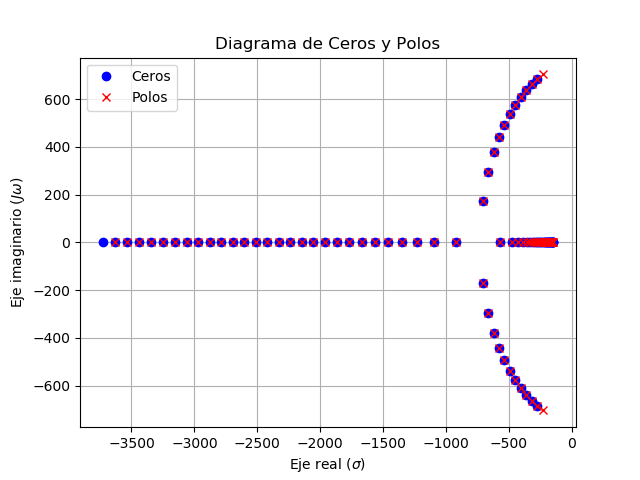
\includegraphics[width=0.7\textwidth]{Imagenes/Zplanepsi.png}
\caption{Diagrama de polos y ceros variando $\psi$ entre 0 y 1.}
	\label{fig:zplanepsi}
\end{figure}

En un ecualizador analógico, al modificar una frecuencia dada, se modifica también su fase. Este es un proceso inevitable, el cual se busca reducir tanto como sea posible, logrando también que produzca el cambio de tono deseado. Esto se garantiza realizando que el sistema sea de fase mínima.
Debido a que, tanto los polos como los ceros del sistema, sin importar el valor de $\psi$, se encuentran en el semiplano izquierdo, se obtiene el menor diagrama de fase posible, en consecuencia, este sistema es de fase mínima.

Si se busca conseguir que el sistema sea de fase no mínima, se debe seleccionar los componentes tales que los ceros se encuentren en el semiplano derecho. Para lograr esto, se propone llevar la (\ref{equ:hs}) sea de la forma

\begin{equation*}
	H(s) = \frac{a S^2 - b S + c}{a S^2 + b S + c}
\end{equation*}

Esto no es posible debido a que los cambios en los componentes modifican también los polos existentes, colocando a estos también en el semiplano derecho, situación que implica que el sistema no sea estable. 

\subsection{Desarrollo del circuito y selección de componentes}
\label{sub:desarrollo}

Teniendo en cuenta lo expresado en la primer sección, se procede a elegir frecuencias de corte para cada una de las instancias. Recordando el que el espectro auditivo del ser humano abarca desde los $20 \ Hz$ a los $20 \ kHz$, y considerando lo mostrado en la Figura (\ref{fig:divfreq}), se decide buscar una frecuencia representativa para cada parte del espectro (bajos, medios y altos). Debido al carácter logarítmico de las frecuencias, se calculan dichos valores de la forma:
\begin{equation*}
	\log{(f_{med})} = \frac{\log(f_{min}) + \log(f_{max})}{2} = \log(\sqrt{f_{min} f_{max}})
	\label{equ:felegida}
\end{equation*}

Es así que se necesita una frecuencia cercana a los $77.50 \ Hz$ para las frecuencias bajas, $1.2 \ kHz$ para las medias y $10 \ kHz$ para las altas. De esta forma, y pensando en valores comerciales de ecualizadores, cuyas amplificaciones varían entre $\pm 12 \ dB$ y $\pm 15 \ dB$, se seleccionan los elementos deseados, completando la siguiente tabla:

\begin{table}[H]
\begin{center}
\begin{tabular}{ccccccc}
\hline
Banda & $R_1$ & $R_2$ & $R_3$ & $C_1$ & $C_2$ & $f_o$ \\
\hline
Baja & $10 \ k\Omega$ & $100 \ k\Omega$ & $1 \ M\Omega$ & $68 \ nF$ & $6.8 \ nF$ & $81.08 \ Hz$ \\
Media & $1 \ k\Omega$ & $10 \ k\Omega$ & $100 \ k\Omega$ & $47 \ nF$ & $4.7 \ nF$ & $1.17 \ kHz$ \\
Alta & $100 \ \Omega$ & $1 \ k\Omega$ & $10 \ k\Omega$ & $56 \ nF$ & $5.6 \ nF$ & $9.85 \ kHz$\\
\hline
\end{tabular}
\caption{Valores de los componentes seleccionados.}
\label{tabla:valores}
\end{center}
\end{table}

Por cuestiones de disponibilidad de componentes, se debió utilizar un potenciómetro $50 \ k\Omega$ ($R_2$) para las frecuencias altas. Para verificar la validez de esto, se debe volver a analizar lo detallado en (\ref{equ:hs}) con las expresiones halladas en el caso más generico, es decir, las representadas en (\ref{equ:general}), ya que no se cumple que $R_3 = 10R_2$. Es por eso que, manteniendo todos los valores expresados en la Tabla (\ref{tabla:valores}), a excepción de $R_2$, y sabiendo que para el caso más genérico la frecuencia de corte viene dada por la expresión
\begin{equation}
	f_o = \frac{1}{2\pi} \cdot \sqrt{\frac{2R_1 + R_2}{\alpha_H}}
	\label{equ:fogeneral}
\end{equation}
se determina la frecuencia de dicha instancia es de $8.96 \ kHz$.

Se podría solventar dicho problema reemplazando $R_3$ por una resistencia de $500 \ k\Omega$ para poder cumplir la condición mencionada. Dicha opción es descartada ya que al realizar esto se observan 2 factores: el primero se encuentra en la frecuencia central del filtro, que al calcularla nuevamente, resulta ser próxima a $1.27 \ kHz$, mientras que el segundo resulta ser la amplificación. Si bien se consigue mayor amplificación, afecta con las demás bandas y además no se cumple con el hecho de respetar los valores de amplificación de ecualizadores comerciales, como se mencionó anteriormente.
\begin{figure}[H]
\centering
	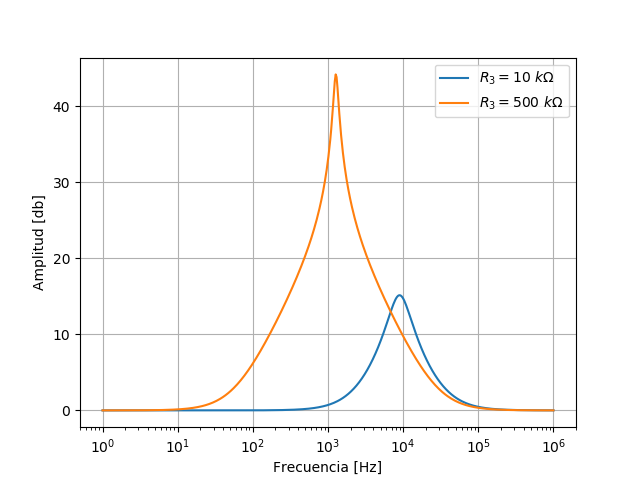
\includegraphics[width=0.7\textwidth]{Imagenes/r3comp.png}
	\caption{Comparación de la transferencia en módulo cambiando $R_3$.}
	\label{fig:r3comp}
\end{figure}

Se destaca el error realizado al obtener las frecuencias finales, las cuales no son exactamente las que se obtuvieron gracias a (\ref{equ:felegida}). Es así que se busca determinar si estas variaciones son aceptables o no. Tomando un error máximo del 5\%, y dado el carácter logarítmico de la audición humana, se calcula el margen máximo y mínimo del error para frecuencia central dada como: 
\begin{equation*}
	\log{(f_{med} \pm \delta)} = \log{(f_{med} \pm f_{med}\cdot 0.05)} = \log{(f_{med} \left(1 \pm 0.05\right))}
\end{equation*}

Es así que se efectúa la siguiente tabla:

\begin{table}[H]
\centering
\begin{tabular}{ccccc}
\hline
\textbf{Banda} & $\mathbf{log(f_{calculada})}$ & $\mathbf{log(f_{calculada} + \delta)}$ & $\mathbf{log(f_{calculada} - \delta)}$ & $\mathbf{log(f_{real})}$ \\
\hline
Baja & 1.89 & 1.91 & 1.87 & 1.91 \\
Media & 3.07 & 3.09 & 3.06 & 3.07 \\
Alta & 4 & 4.02 & 3.97 & 3.95 \\
\hline
\end{tabular}
\caption{Margenes de errores máximos y mínimos de las frecuencias centrales.}
\label{tabla:errores}
\end{table}

Se concluye que las frecuencias elegidas son aceptables para la tolerancia seleccionada, salvo por la elegida para representar la banda de las altas. En este caso, se está cometiendo un error del 10\%, el cual, si bien no respeta el límite que se había propuesto, se realiza una excepción por las razones previamente explicadas y expuestas en la Figura (\ref{fig:r3comp}), tomando este margen como aceptable. 

Una vez determinado esto, se optó por colocar las tres instancias en serie, ya que de esta forma se aprovecha mejor la amplificación de cada una, debido a la alta impedancia de entrada del circuito total, razón que se expone más adelante. Otra ventaja que presenta esta disposición es la facilidad al calcular tanto la transferencia del circuito, ya que debido a teoría de cuadripolos, esta resulta del producto de la de cada etapa, obtenida de reemplazar los valores mostrados en la Tabla (\ref{tabla:valores}) en (\ref{equ:hs}). Es así que se deja en forma de ecuación lo dicho anteriormente:

\begin{equation}
	H(S) = H_{bajas}(S) \cdot H_{medias}(S) \cdot H_{altas}(S)
\end{equation}
siendo el subindice representativo de las frecuencias que modifican.

Es así que se procede a graficar la respuesta en frecuencia calculada de todo el circuito, variando el factor $\psi$ para una instancia por vez, fijando los demás en $0.5$.
\begin{figure}[H]
\centering
	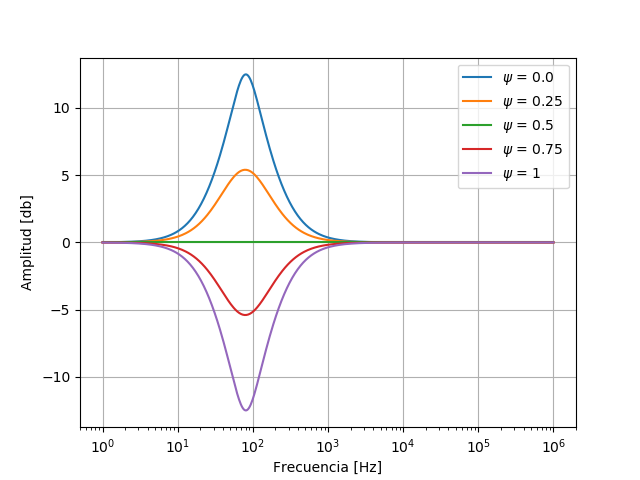
\includegraphics[width=0.7\textwidth]{Imagenes/Low-psi-bode.png}
	\caption{Diagrama de Bode en amplitud, variando $\psi$ de las frecuencias bajas.}
	\label{fig:bode_modulo_low}
\end{figure}
\begin{figure}[H]
\centering
	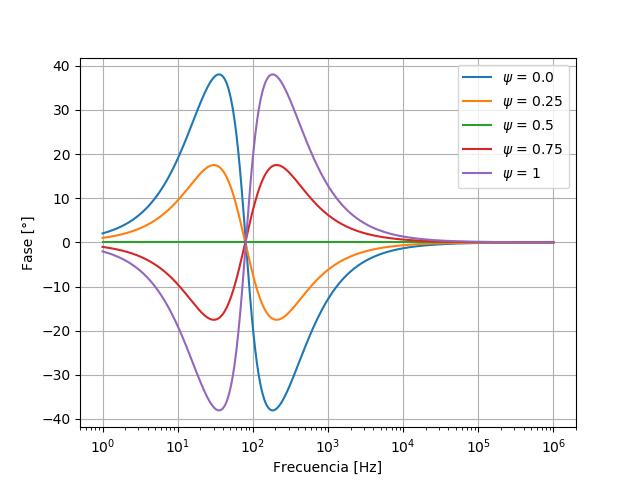
\includegraphics[width=0.7\textwidth]{Imagenes/Low-psi-ph.png}
	\caption{Diagrama de Bode en fase, variando $\psi$ de las frecuencias bajas.}
	\label{fig:bode_ph_low}
\end{figure}
\begin{figure}[H]
\centering
	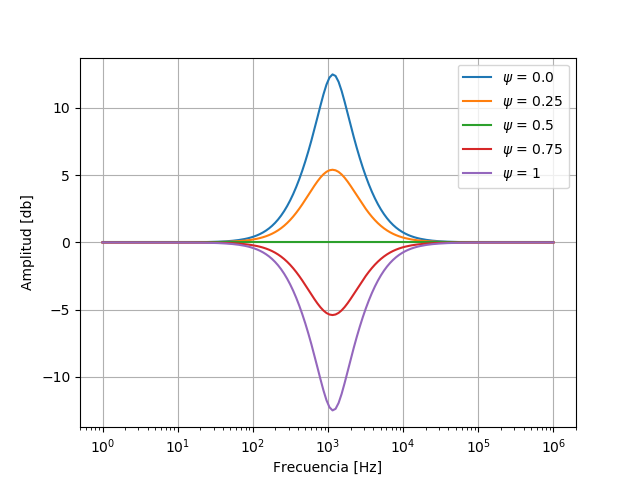
\includegraphics[width=0.7\textwidth]{Imagenes/Medium-psi-bode.png}
	\caption{Diagrama de Bode en amplitud, variando $\psi$ de las frecuencias medias.}
	\label{fig:bode_modulo_med}
\end{figure}
\begin{figure}[H]
\centering
	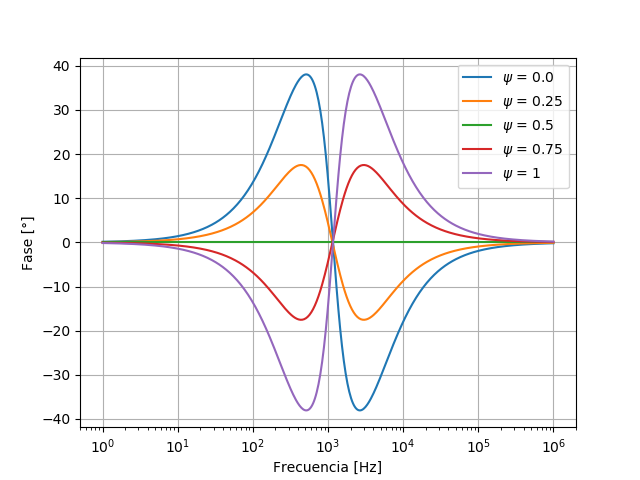
\includegraphics[width=0.7\textwidth]{Imagenes/Medium-psi-ph.png}
	\caption{Diagrama de Bode en fase, variando $\psi$ de las frecuencias medias.}
	\label{fig:bode_ph_med}
\end{figure}
\begin{figure}[H]
\centering
	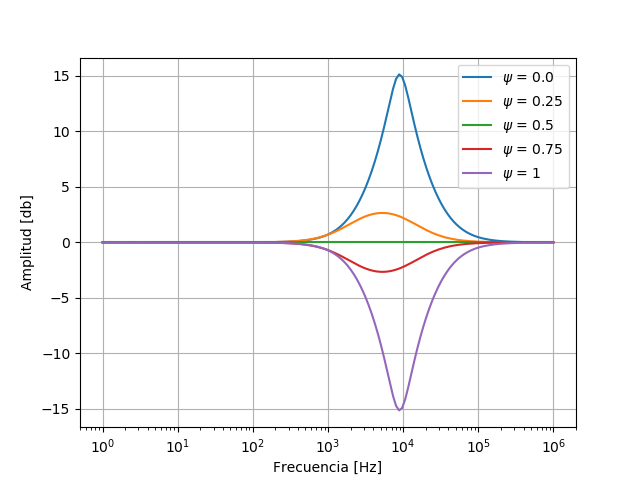
\includegraphics[width=0.7\textwidth]{Imagenes/High-psi-bode.png}
	\caption{Diagrama de Bode en amplitud, variando $\psi$ de las frecuencias altas.}
	\label{fig:bode_modulo_high}
\end{figure}
\begin{figure}[H]
\centering
	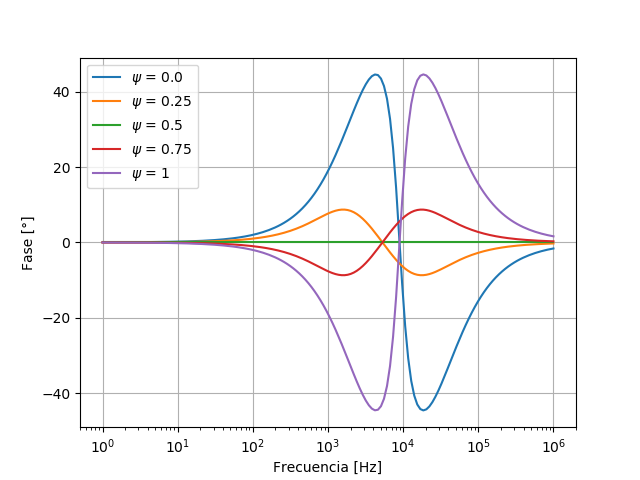
\includegraphics[width=0.7\textwidth]{Imagenes/High-psi-ph.png}
	\caption{Diagrama de Bode en fase, variando $\psi$ de las frecuencias altas.}
	\label{fig:bode_ph_high}
\end{figure}

Es así que se observa que cada instancia genera un cambio en la ganancia similar, en torno a la frecuencia seleccionada en la Tabla (\ref{tabla:valores}). De la misma forma se da en los cambios de fase.
%Cabe destacar el oído humano no detecta cambios en la fase, debido a que no posee forma de comparar dicha variación, es decir, no cuenta con una referencia con la cual contrastar el desfasaje.
%Se puede hacer un detenimiento en las bandas que se encuentran en el entorno de la frecuencia de corte en las Figuras (\ref{fig:bode_ph_low}), (\ref{fig:bode_ph_med}) y (\ref{fig:bode_ph_high}), pero dicho intervalo sigue siendo lo suficientemente grande como para ser detectado por el oído humano.
También, resulta pertinente destacar los corrimientos que se producen tanto en la fase como en la amplitud al variar las altas frecuencias, lo cual se debe al cambio realizado del potenciómetro. En otras palabras, la causa de este fenómeno se debe a que la condición de que $R_3 = 10R_2$ deja de ser valida.

%De la misma forma, se muestra la impedancia de entrada en función de la frecuencia para el circuito total, variando $\psi$ para una instancia y fijando las demás en $0.5$.
%\begin{figure}[H]
%\centering
%	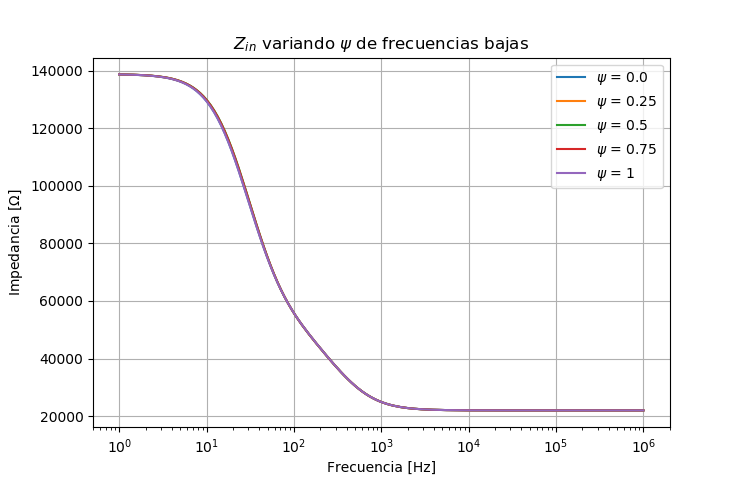
\includegraphics[width=0.7\textwidth, trim = {0 0 0 1.35cm}, clip]{Imagenes/Zin-Low-Mod.png}
%	\caption{Impedancia de entrada en modulo, variando $\psi$ para las frecuencias bajas.}
%	\label{fig:zin_modulo_low}
%\end{figure}
%\begin{figure}[H]
%\centering
%	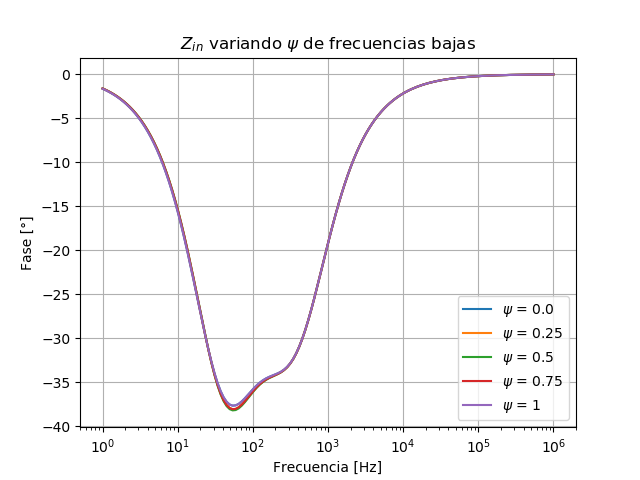
\includegraphics[width=0.7\textwidth, trim = {0 0 0 1.35cm}, clip]{Imagenes/Zin-Low-Ph.png}
%	\caption{Fase de la impedancia de entrada, variando $\psi$ para las frecuencias bajas.}
%	\label{fig:zin_ph_low}
%\end{figure}
%\begin{figure}[H]
%\centering
%	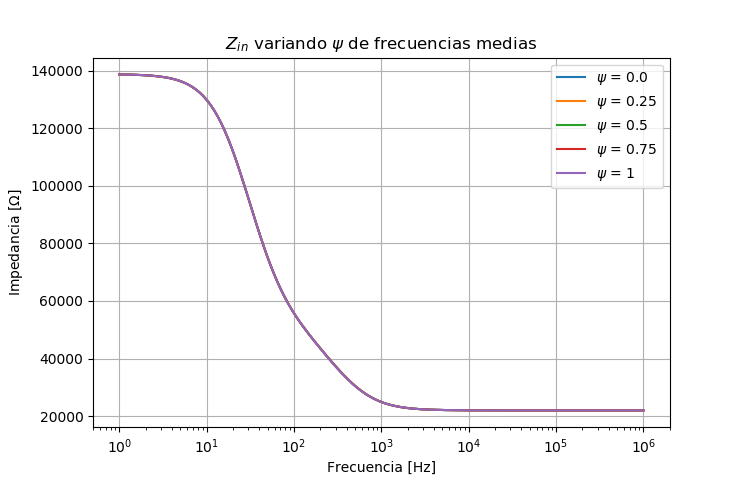
\includegraphics[width=0.7\textwidth, trim = {0 0 0 1.35cm}, clip]{Imagenes/Zin-Med-Mod.png}
%	\caption{Impedancia de entrada en modulo, variando $\psi$ para las frecuencias medias.}
%	\label{fig:zin_modulo_med}
%\end{figure}
%\begin{figure}[H]
%\centering
%	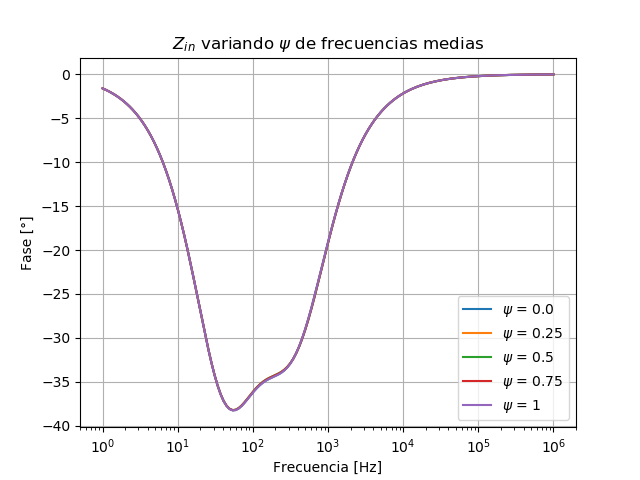
\includegraphics[width=0.7\textwidth, trim = {0 0 0 1.35cm}, clip]{Imagenes/Zin-Med-Ph.png}
%	\caption{Fase de la impedancia de entrada, variando $\psi$ para las frecuencias medias.}
%	\label{fig:zin_ph_med}
%\end{figure}
%\begin{figure}[H]
%\centering
%	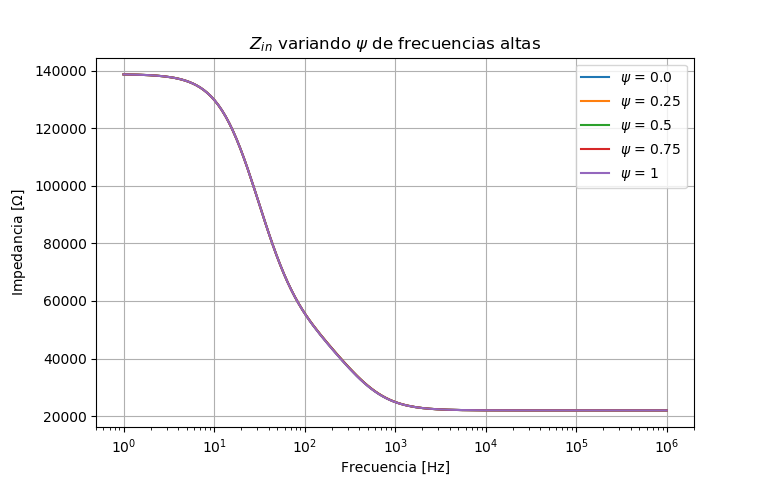
\includegraphics[width=0.7\textwidth, trim = {0 0 0 1.35cm}, clip]{Imagenes/Zin-High-Mod.png}
%	\caption{Impedancia de entrada en modulo, variando $\psi$ para las frecuencias altas.}
%	\label{fig:zin_modulo_high}
%\end{figure}
%\begin{figure}[H]
%\centering
%	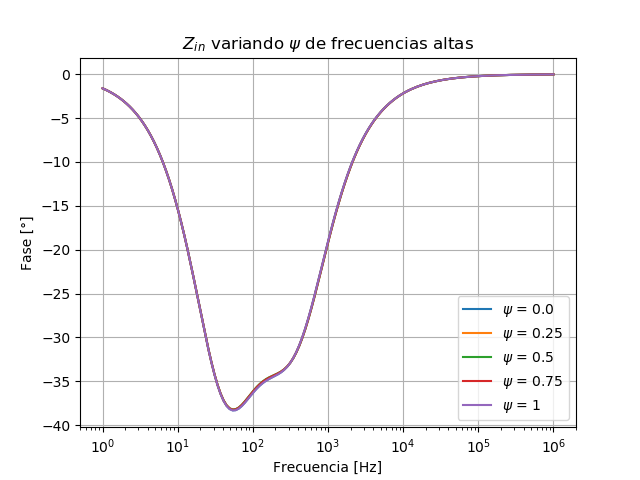
\includegraphics[width=0.7\textwidth, trim = {0 0 0 1.35cm}, clip]{Imagenes/Zin-High-Ph.png}
%	\caption{Fase de la impedancia de entrada, variando $\psi$ para las frecuencias altas.}
%	\label{fig:zin_ph_high}
%\end{figure}

Simulando la impedancia de entrada se obtiene que esta permanece prácticamente constante frente a cambios en $\psi$ de cualquier etapa, es por eso que se grafica esta variable a continuación para todo el sistema una única vez:

\begin{figure}[H]
\centering
	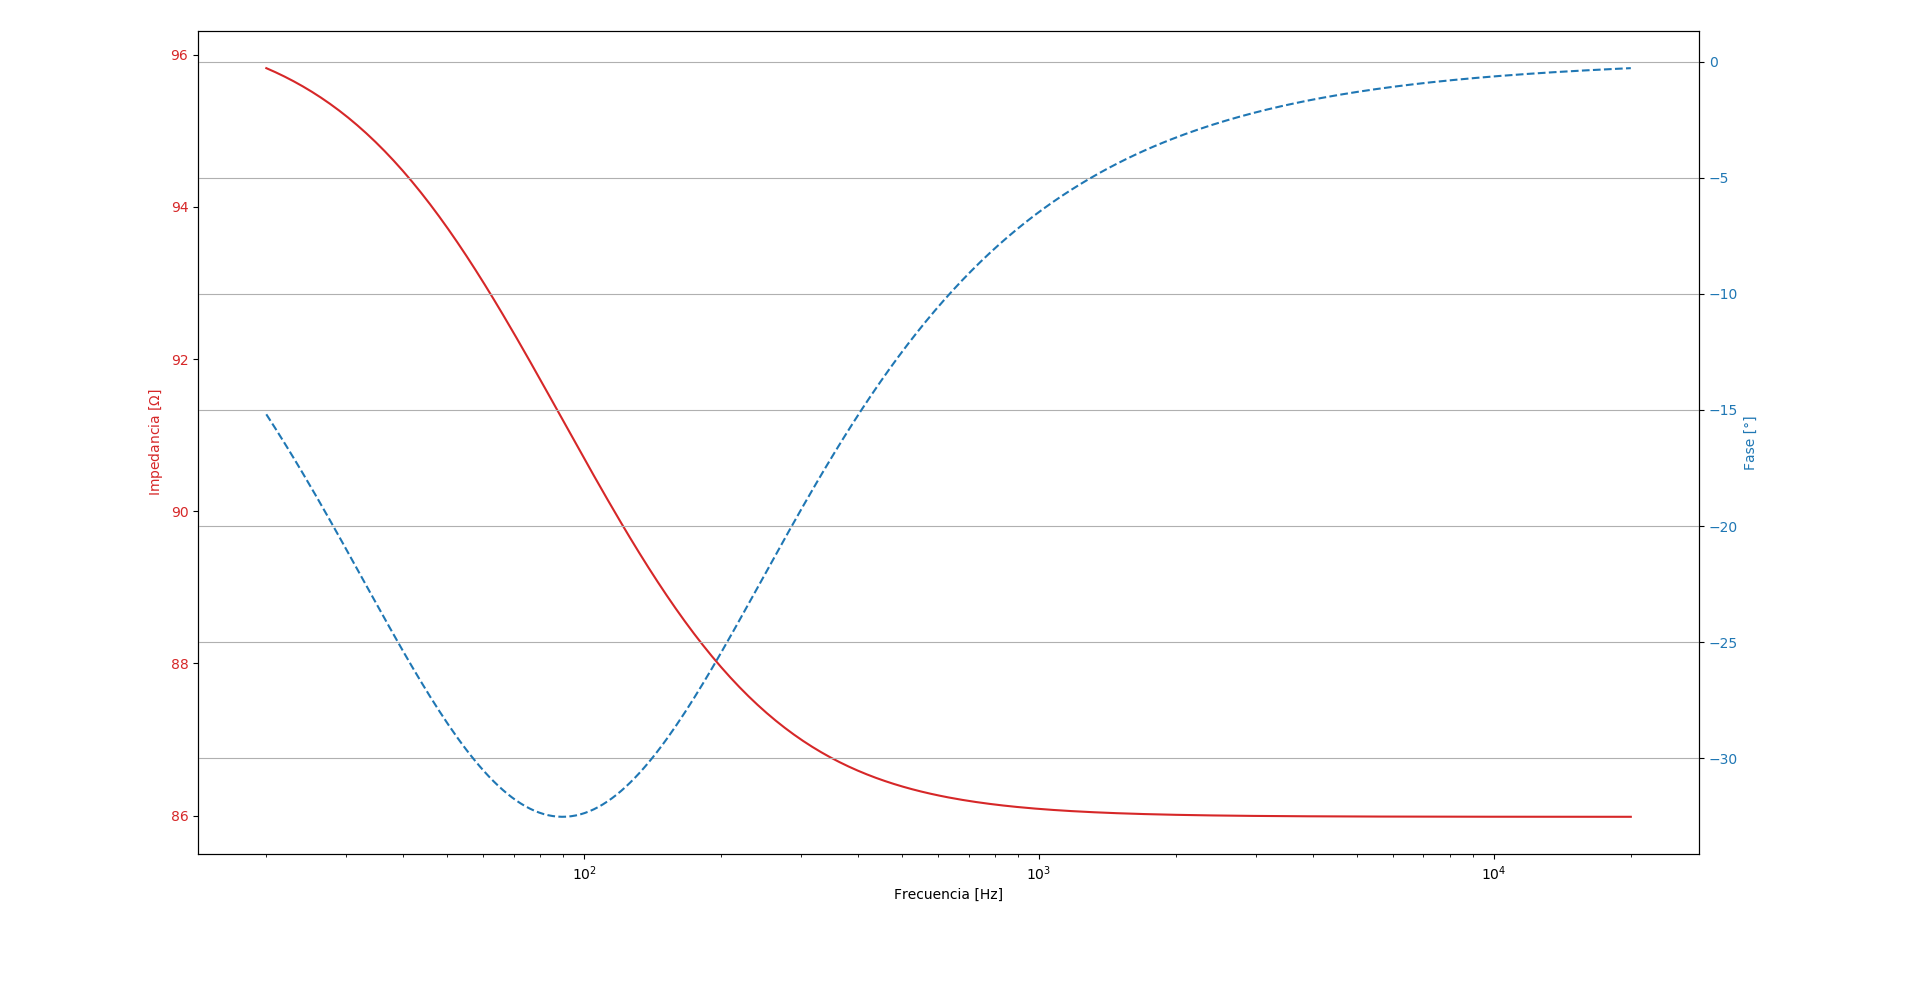
\includegraphics[width=0.9\textwidth]{Imagenes/Zin.png}
	\caption{Impedancia de entrada en modulo (en rojo) y fase (en azul).}
	\label{fig:zin}
\end{figure}

Se observa de esta figura que la impedancia de entrada se comporta de manera resistiva a altas frecuencias, mientras que en las bajas y medias comienza a verse un efecto capacitivo, sin llegar a ser este más grande que el resistivo. Como se mencionó anteriormente, presentar cada instancia en serie es más conveniente que en paralelo, debido a la variable previamente analizada. Esto se observa en las Figuras (\ref{fig:zin_comp_mod}) y (\ref{fig:zin_comp_ph}). La impedancia de entrada en la disposición en paralelo se obtiene justamente del paralelo de la de cada instancia, siendo esta menor que la seleccionada. Es así que se aprovecha mejor la disposición en serie que en paralelo. 
\begin{figure}[H]
\centering
	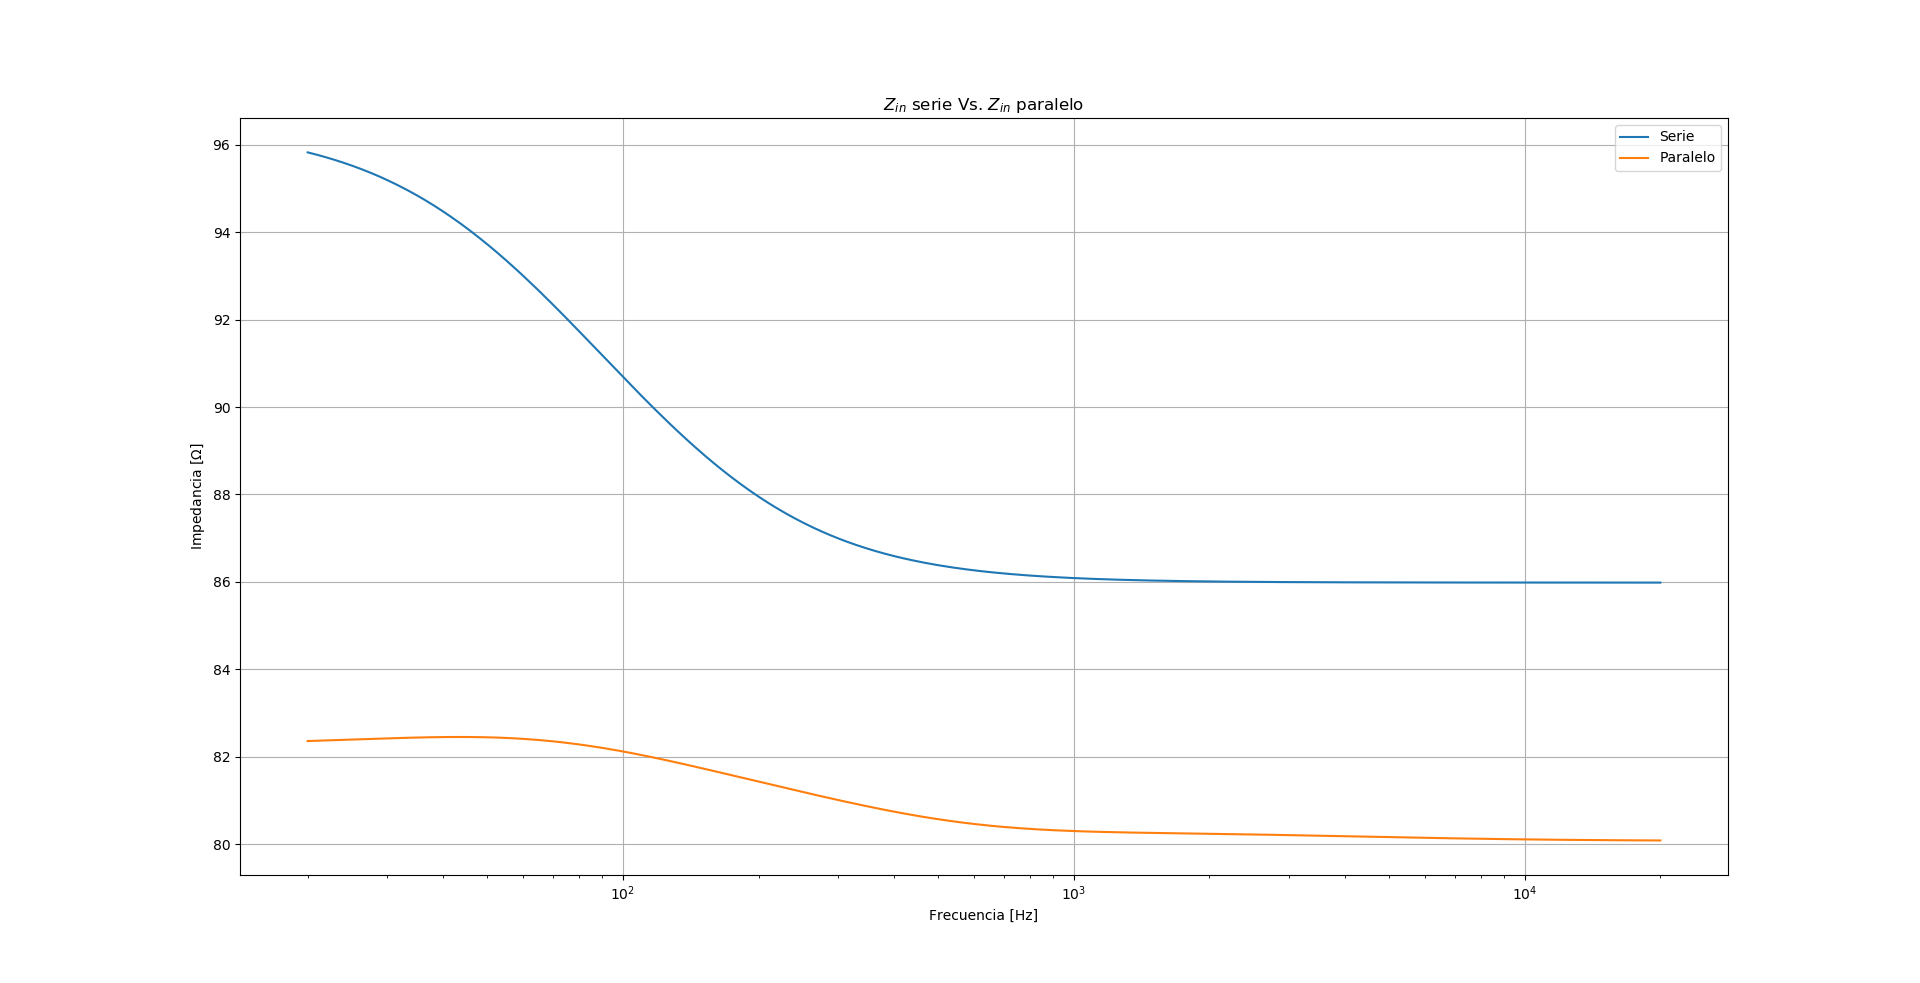
\includegraphics[width=0.9\textwidth, trim = {0 0 0 1.35cm}, clip]{Imagenes/Z-Paralelo-Vs-Serie-Mod.png}
	\caption{Comparación de impedancias de entrada, en módulo.}
	\label{fig:zin_comp_mod}
\end{figure}
\begin{figure}[H]
\centering
		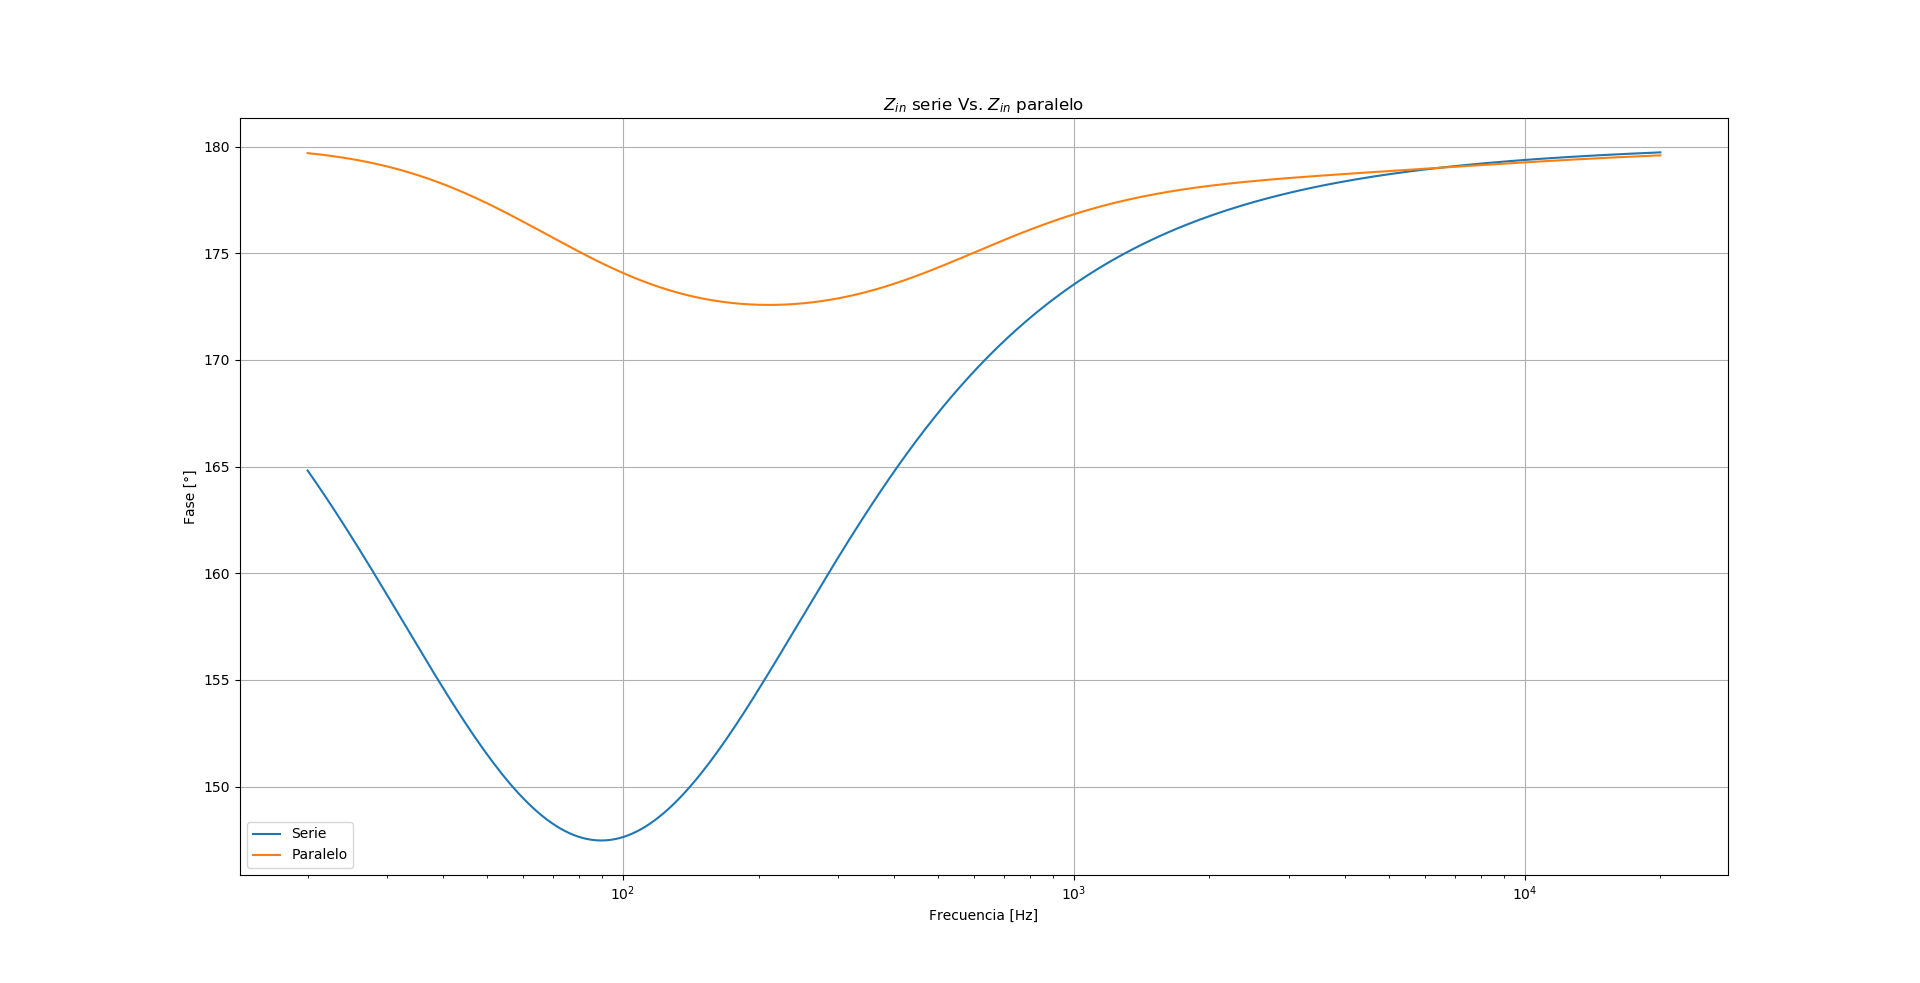
\includegraphics[width=0.9\textwidth, trim = {0 0 0 1.35cm}, clip]{Imagenes/Z-Paralelo-Vs-Serie-Ph.png}
	\caption{Comparación de impedancias de entrada, en fase.}
	\label{fig:zin_comp_ph}
\end{figure}

Cabe aclarar que a la salida del circuito se colocó un capacitor de $220 \ nF$ para eliminar un pequeño offset existente, proveniente de la salida de los operacionales (del orden de los milivolts). Por lo tanto, la impedancia de salida del circuito termina siendo la de dicho capacitor.

De la misma forma que realizó para la impedancia de entrada, se presenta a continuación la de salida:
\begin{figure}[H]
\centering
	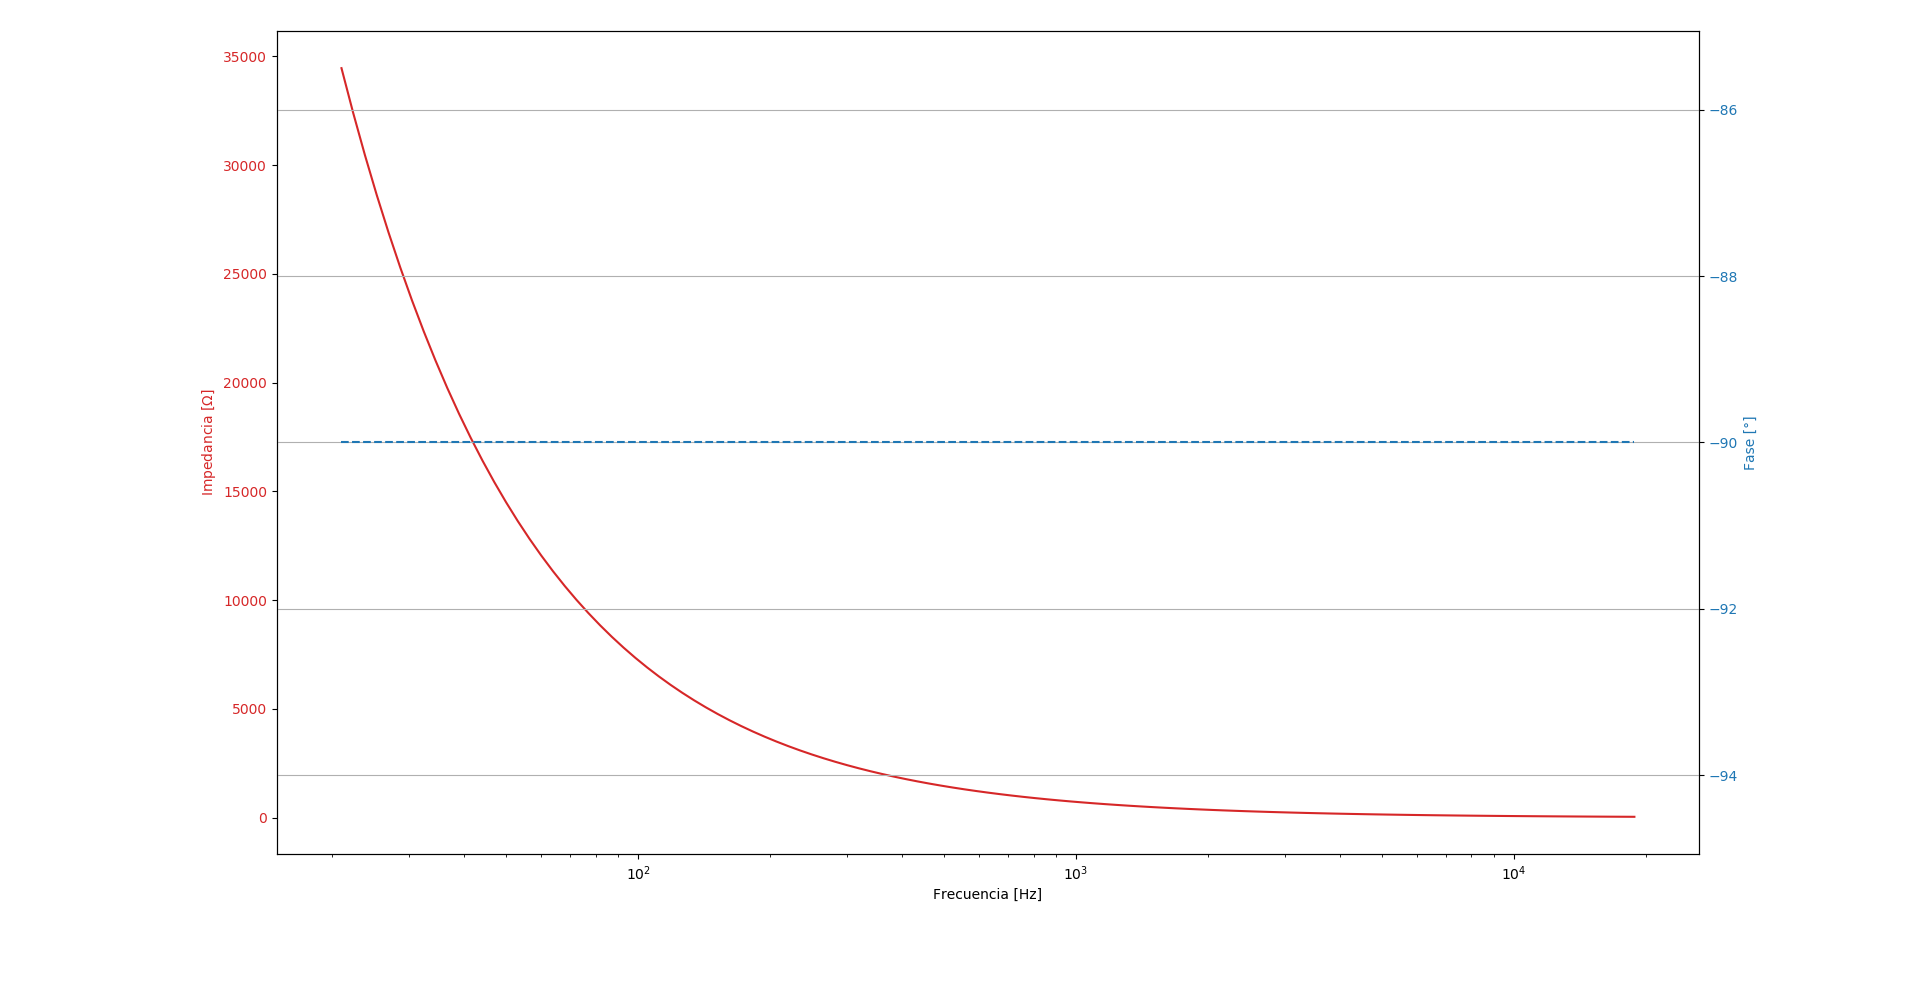
\includegraphics[width=0.9\textwidth]{Imagenes/Zout.png}
	\caption{Impedancia de salida en modulo (en rojo) y fase (en azul).}
	\label{fig:zout}
\end{figure}

Luego, para evitar enfrentarse a amplias variaciones en cuanto a los modelos presentados anteriormente, se decide utilizar tecnología SMD tanto para las resistencias fijas como para los capacitores. De esta forma, y valiéndose del análisis de Montecarlo del programa LTSpice, se obtiene el sigueinte diagrama de Bode, siendo la tolerancia de los componentes mencionados anteriormente de 1 \%.

\begin{figure}[H]	
	\centering
	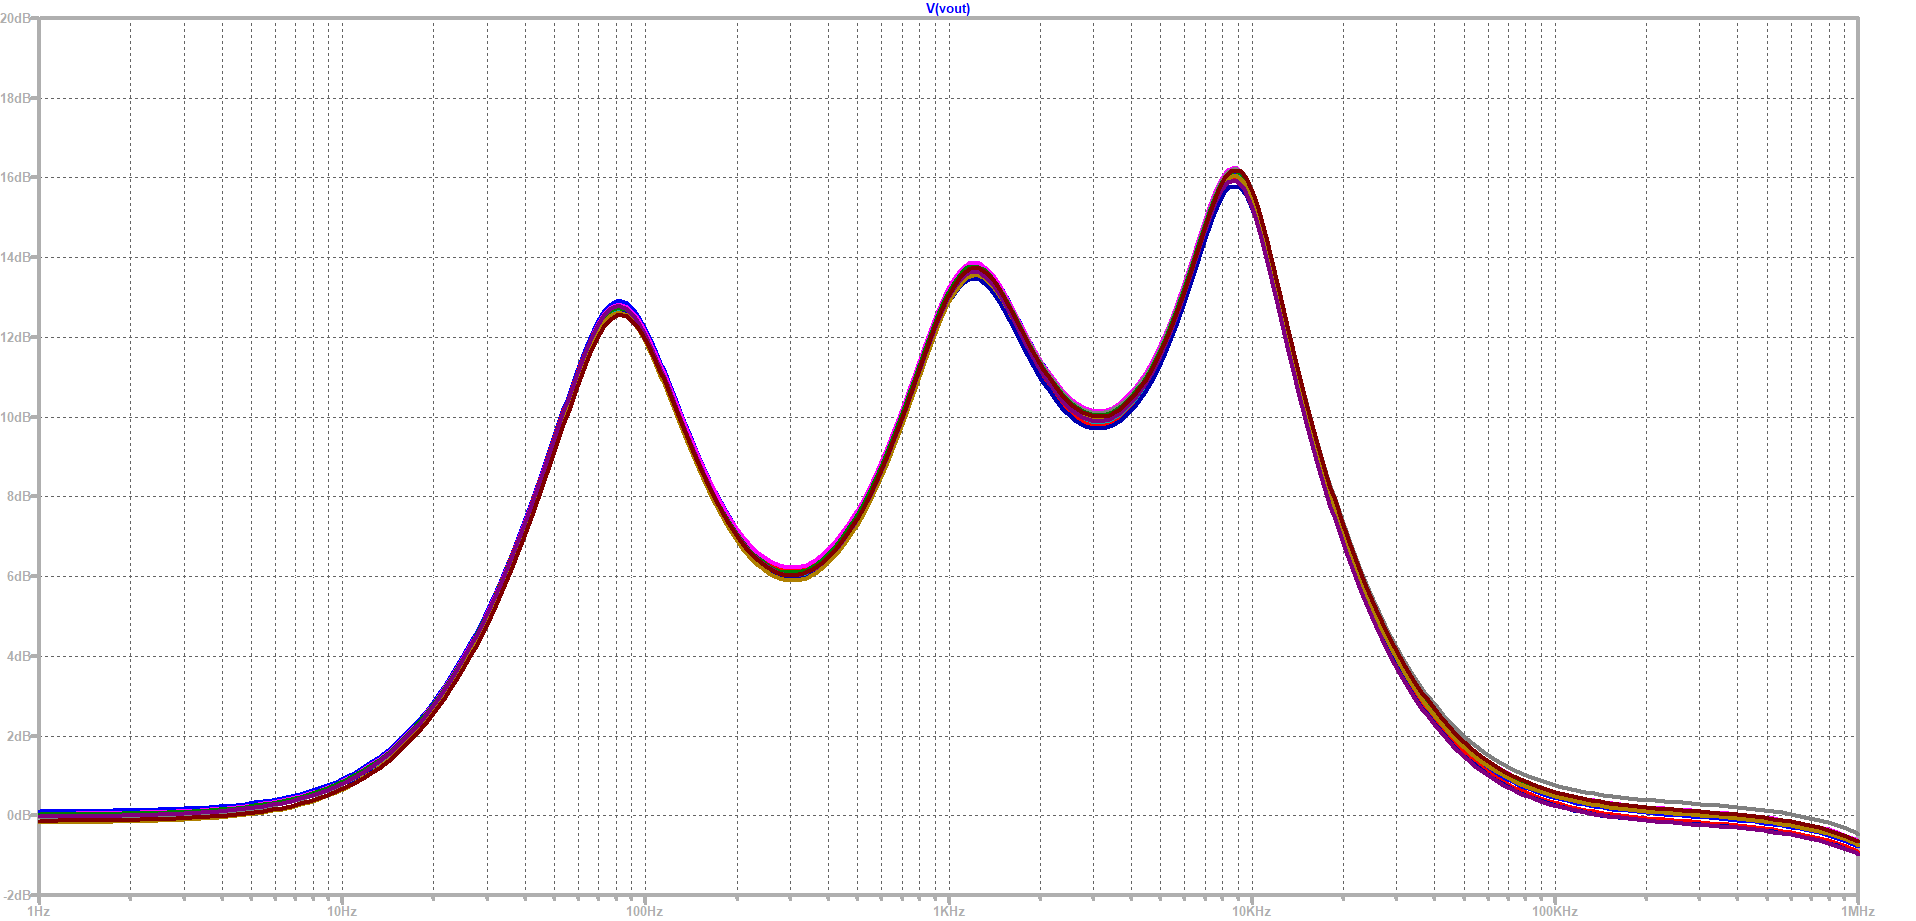
\includegraphics[width=0.7\textwidth]{Imagenes/MC-Mod.png}
	\caption{Análisis de Montecarlo del diagrama de Bode en amplitud.}
	\label{fig:MC-Mod}
\end{figure}

\begin{figure}[H]	
	\centering
	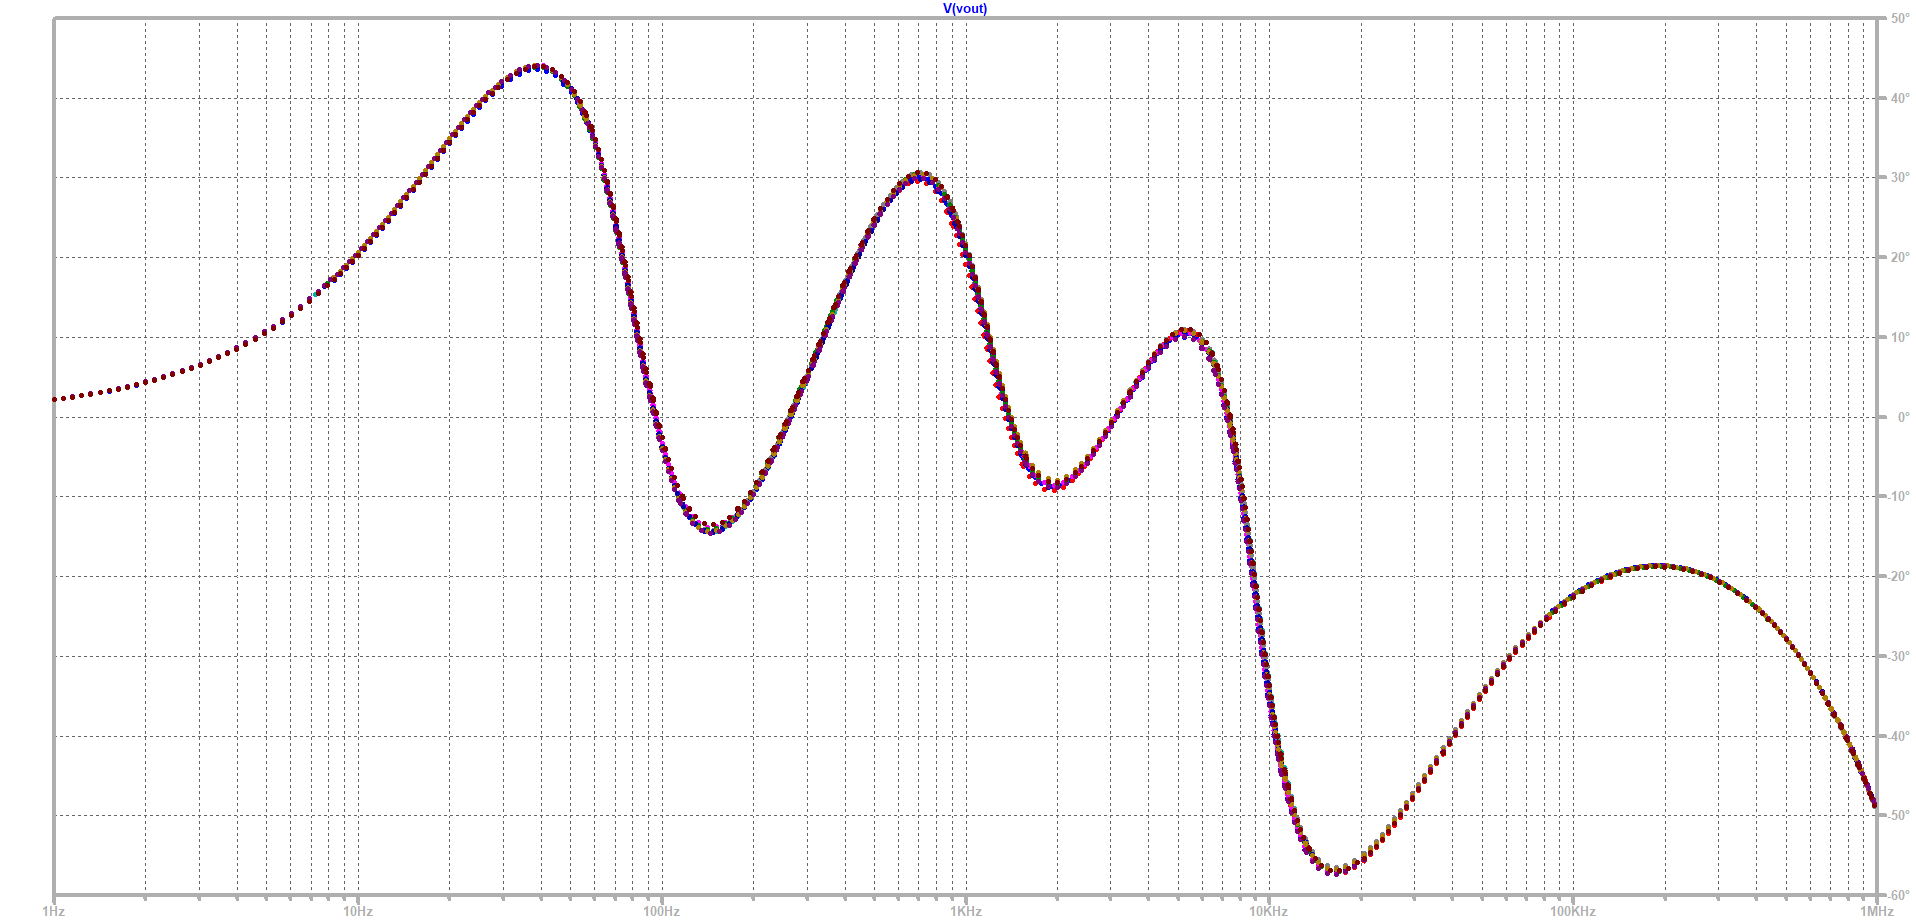
\includegraphics[width=0.7\textwidth]{Imagenes/MC-Ph.png}
	\caption{Análisis de Montecarlo del diagrama de Bode en fase.}
	\label{fig:MC-Ph}
\end{figure}

Como era de esperarse, se consigue que la variación en el Bode simulado sea mínima, debido a las tolerancias elegidas.

\subsection{Resultados obtenidos}

Hasta ahora se han presentado diagramas de Bode y de impedancias de entrada teóricos y simulados. En esta sección se procede a comparar los resultados ya observados en contraste con análisis de las mismas variables pero esta vez, resultantes de simulaciones en LTSpice y mediciones. Para ello se decide fijar para cada etapa un valor de $\psi$ y presentar dicho resultado.

Cabe destacar que para el desarrollo de este circuito se optó utilizar el amplificador operacional \href{http://www.ti.com/lit/ds/symlink/lm833-n.pdf}{LM833}, debido a su frecuente uso en lo que a audio respecta, su bajo ruido de entrada y su amplia ganancia de banda pasante, la cual cubre el espectro audible\footnote{Texas Instruments, ``LM833-N Dual Audio Operational Amplifier'', LM833 datasheet, Mayo 2004 [Revisado Mayo 2012].}. Debido a que este dispositivo es dual y que se requiere un total de tres amplificadores, se utilizan dos LM833, dejando un operacional sin usar. Para aprovecharlo, se decide colocar este último amplificador a la salida del circuito, conectado como un inversor con un potenciómetro, para de esta forma utilizarlo como un controlador de volumen. Por lo tanto, de ahora en más se considera el cambio de fase que este provee al circuito junto con la impedancia que este agrega.   

\subsubsection{Comparaciones}

A continuación, se procede a presentar diagramas de Bode teóricos, simulados y medidos. Para ello, al momento de graficar los resultados teóricos, se fijaron ciertos valores del factor $\psi$ de cada etapa que represente la posición del potenciómetro en el modelo físico, siendo $\psi = 0$ amplificación total y $\psi = 1$ atenuación total. Es así que se obtuvieron los siguientes gráficos.
\begin{figure}[H]	
	\centering
	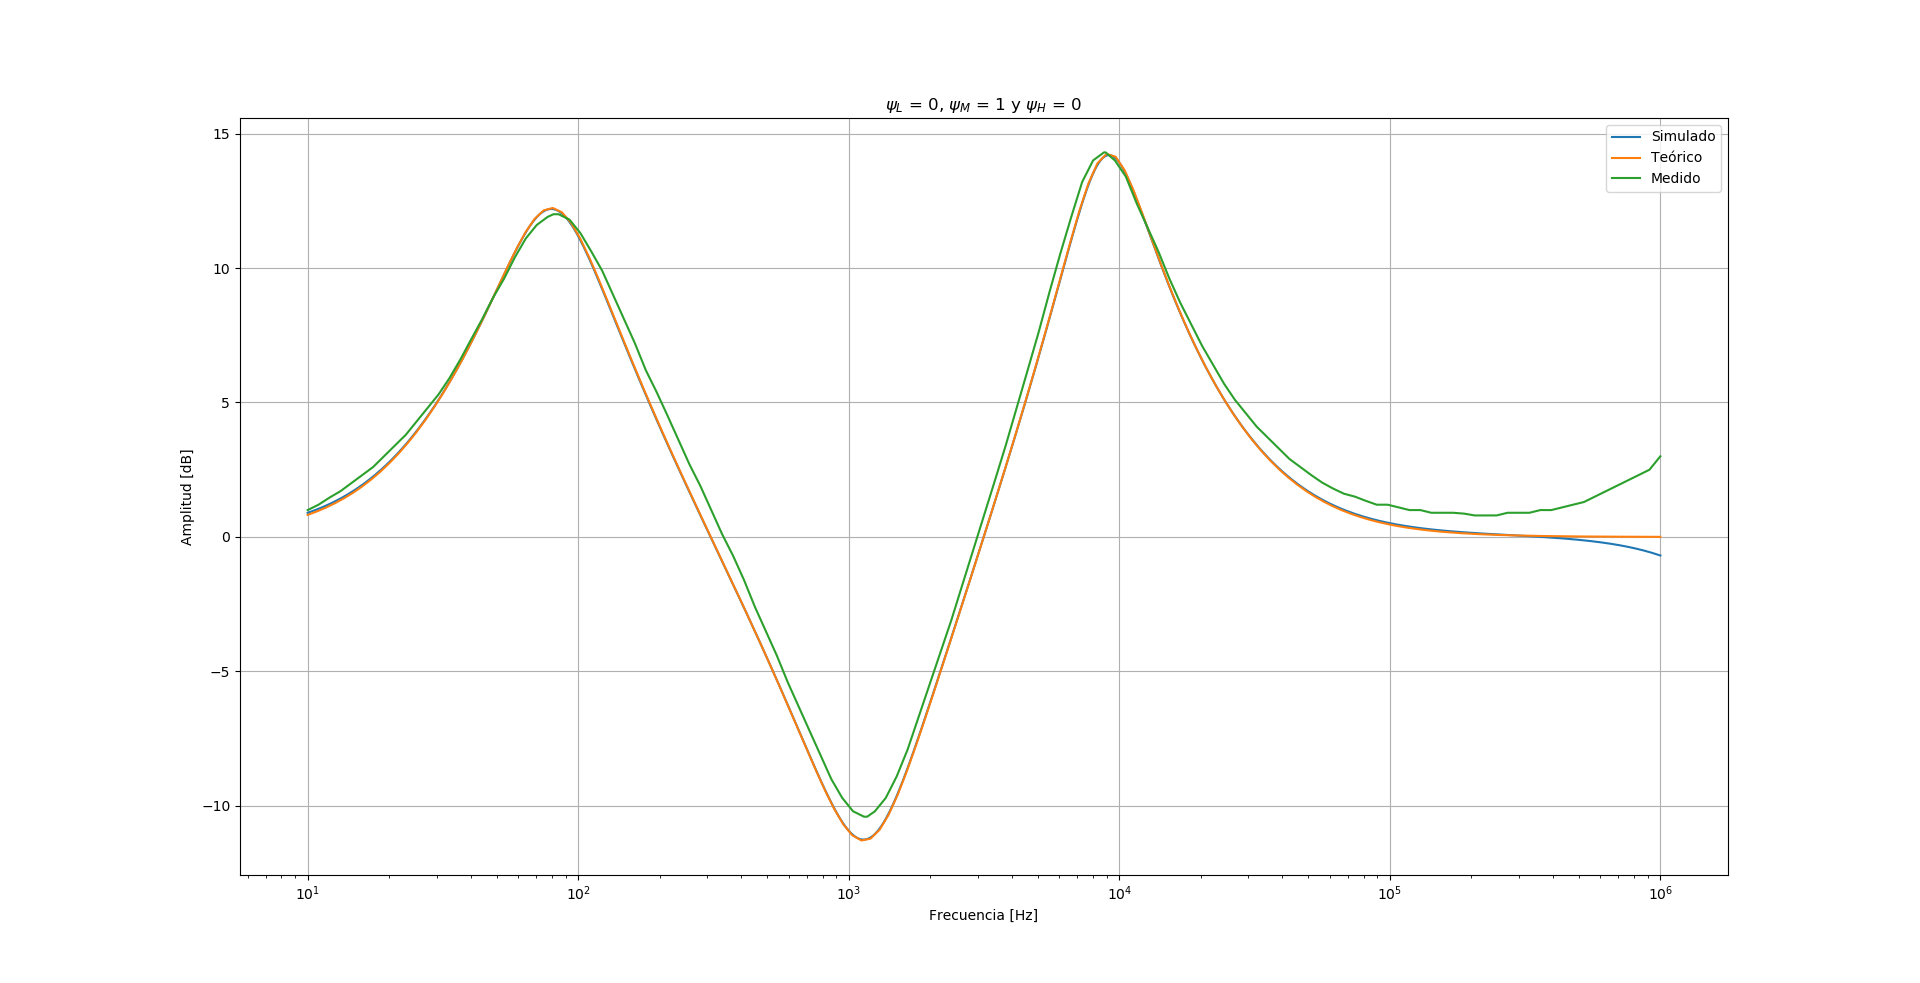
\includegraphics[width=0.9\textwidth]{Imagenes/CBodes-Mod-1.png}
	\caption{Diagrama de Bode en amplitud de la primer medición.}
	\label{fig:CBodes-Mod-1}
\end{figure}
\begin{figure}[H]	
	\centering
	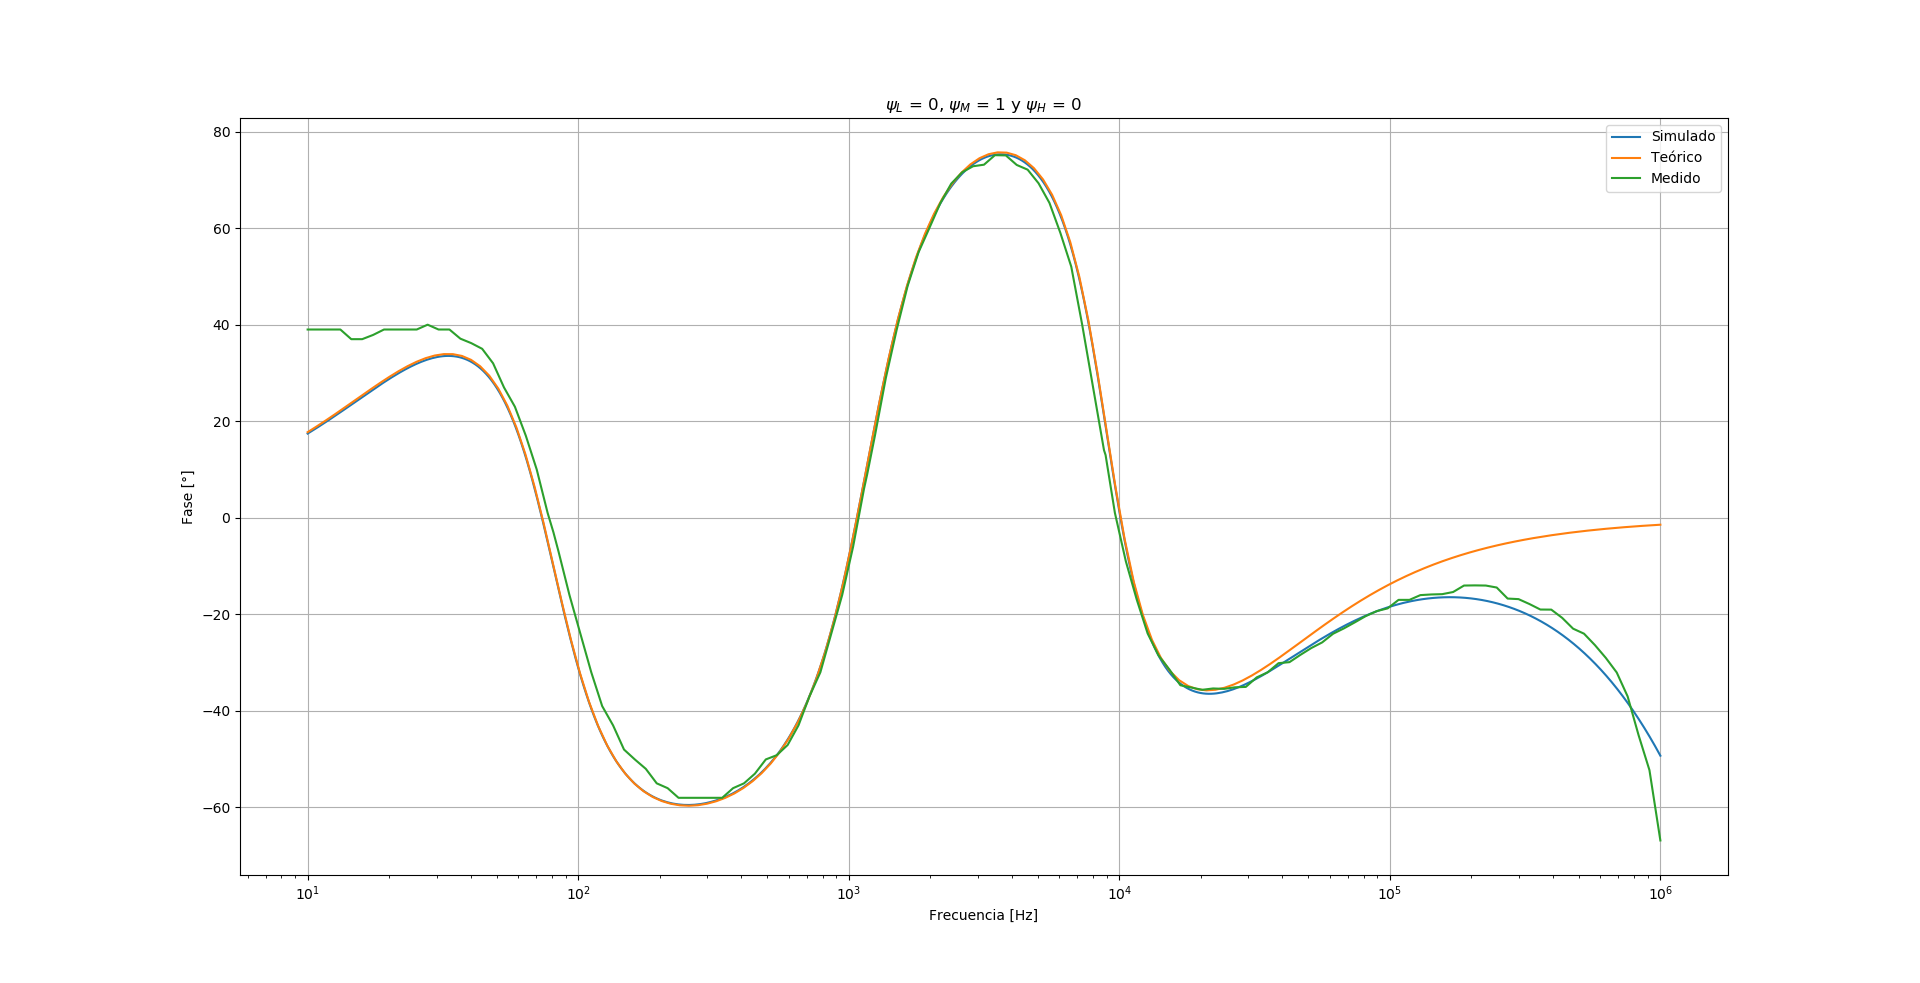
\includegraphics[width=0.9\textwidth]{Imagenes/CBodes-Ph-1.png}
	\caption{Diagrama de Bode en fase de la primer medición.}
	\label{fig:CBodes-Ph-1}
\end{figure}
\begin{figure}[H]	
	\centering
	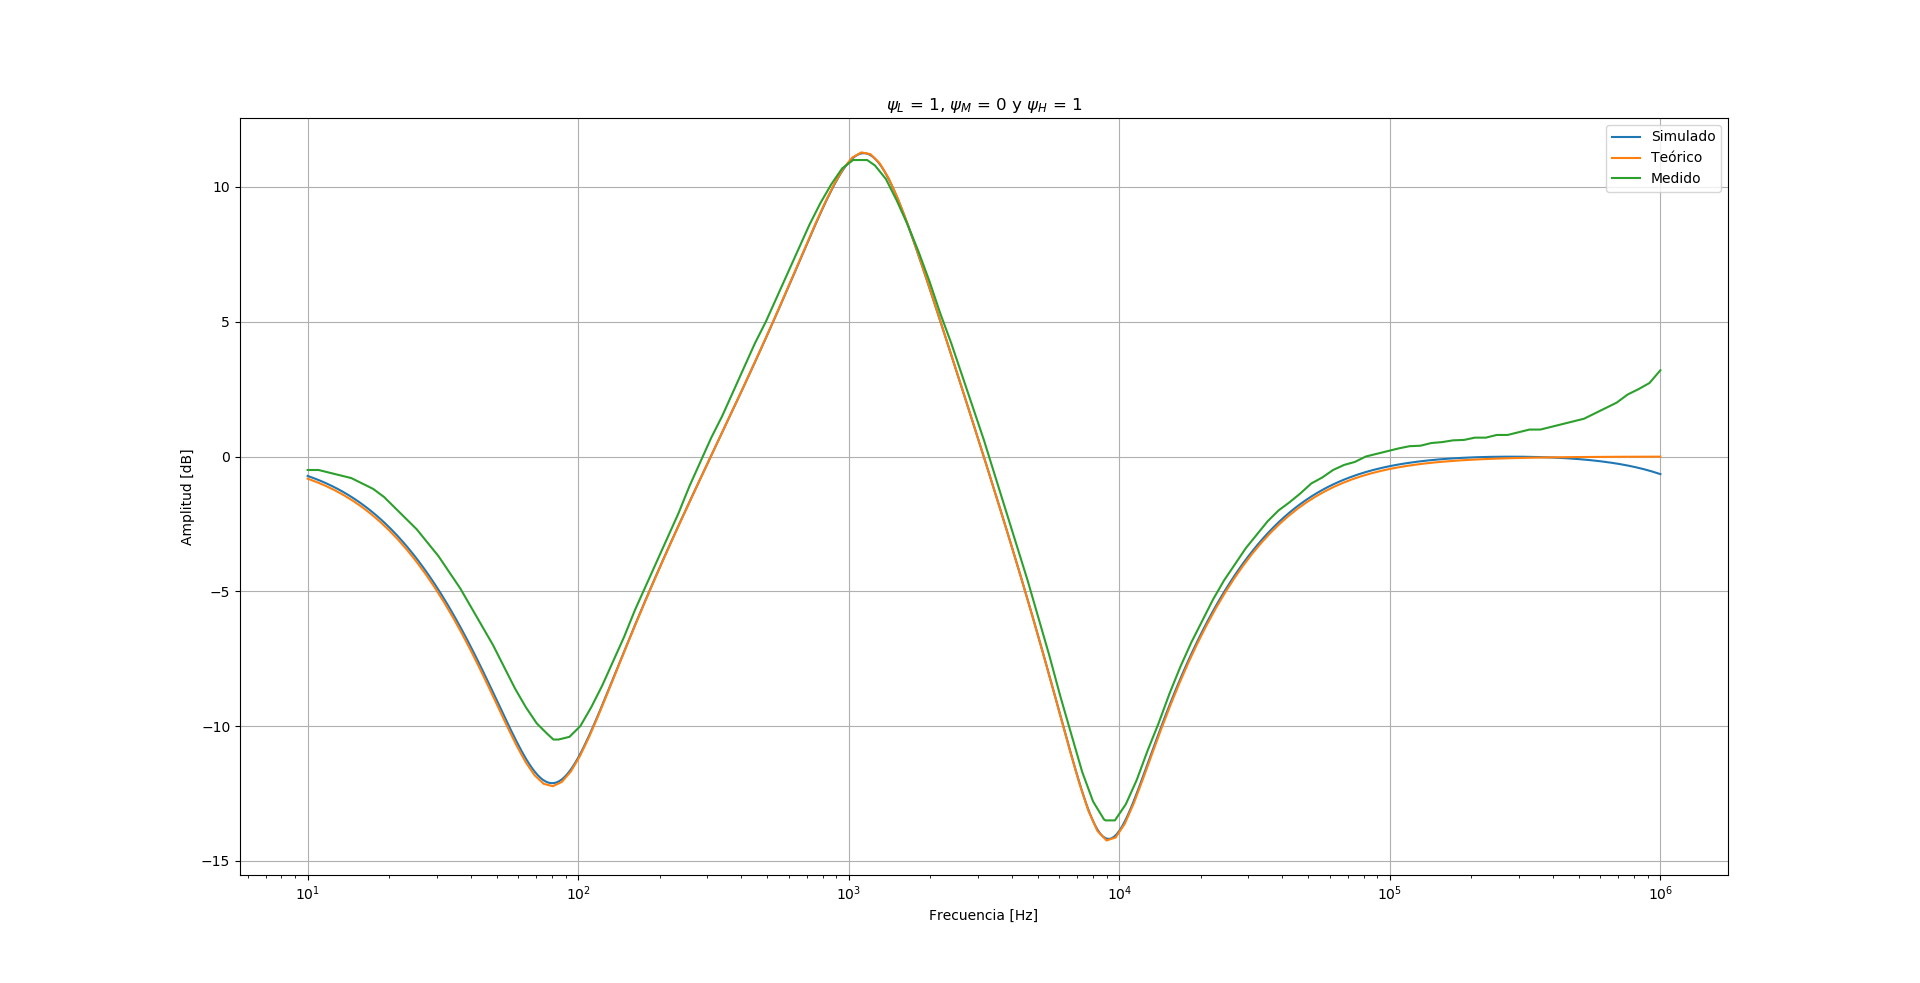
\includegraphics[width=0.9\textwidth]{Imagenes/CBodes-Mod-2.png}
	\caption{Diagrama de Bode en amplitud de la segunda medición.}
	\label{fig:CBodes-Mod-2}
\end{figure}
\begin{figure}[H]	
	\centering
	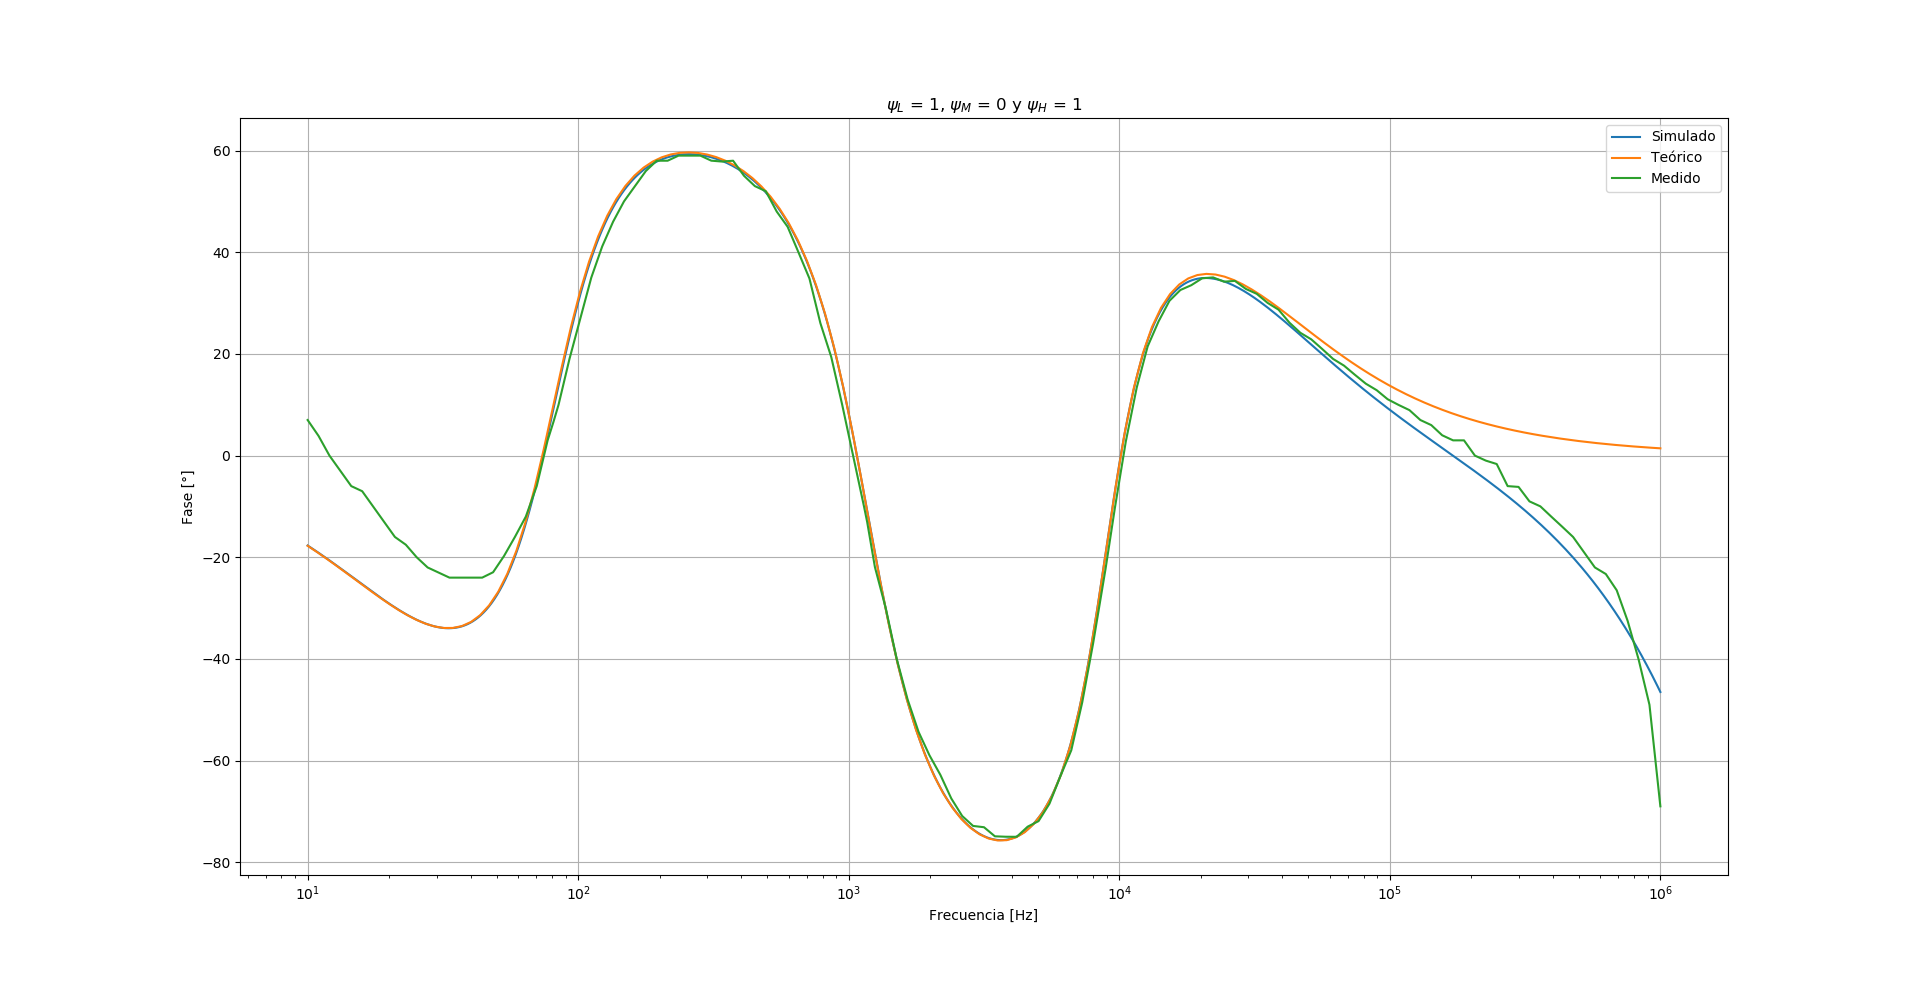
\includegraphics[width=0.9\textwidth]{Imagenes/CBodes-Ph-2.png}
	\caption{Diagrama de Bode en fase de la segunda medición.}
	\label{fig:CBodes-Ph-2}
\end{figure}
\begin{figure}[H]	
	\centering
	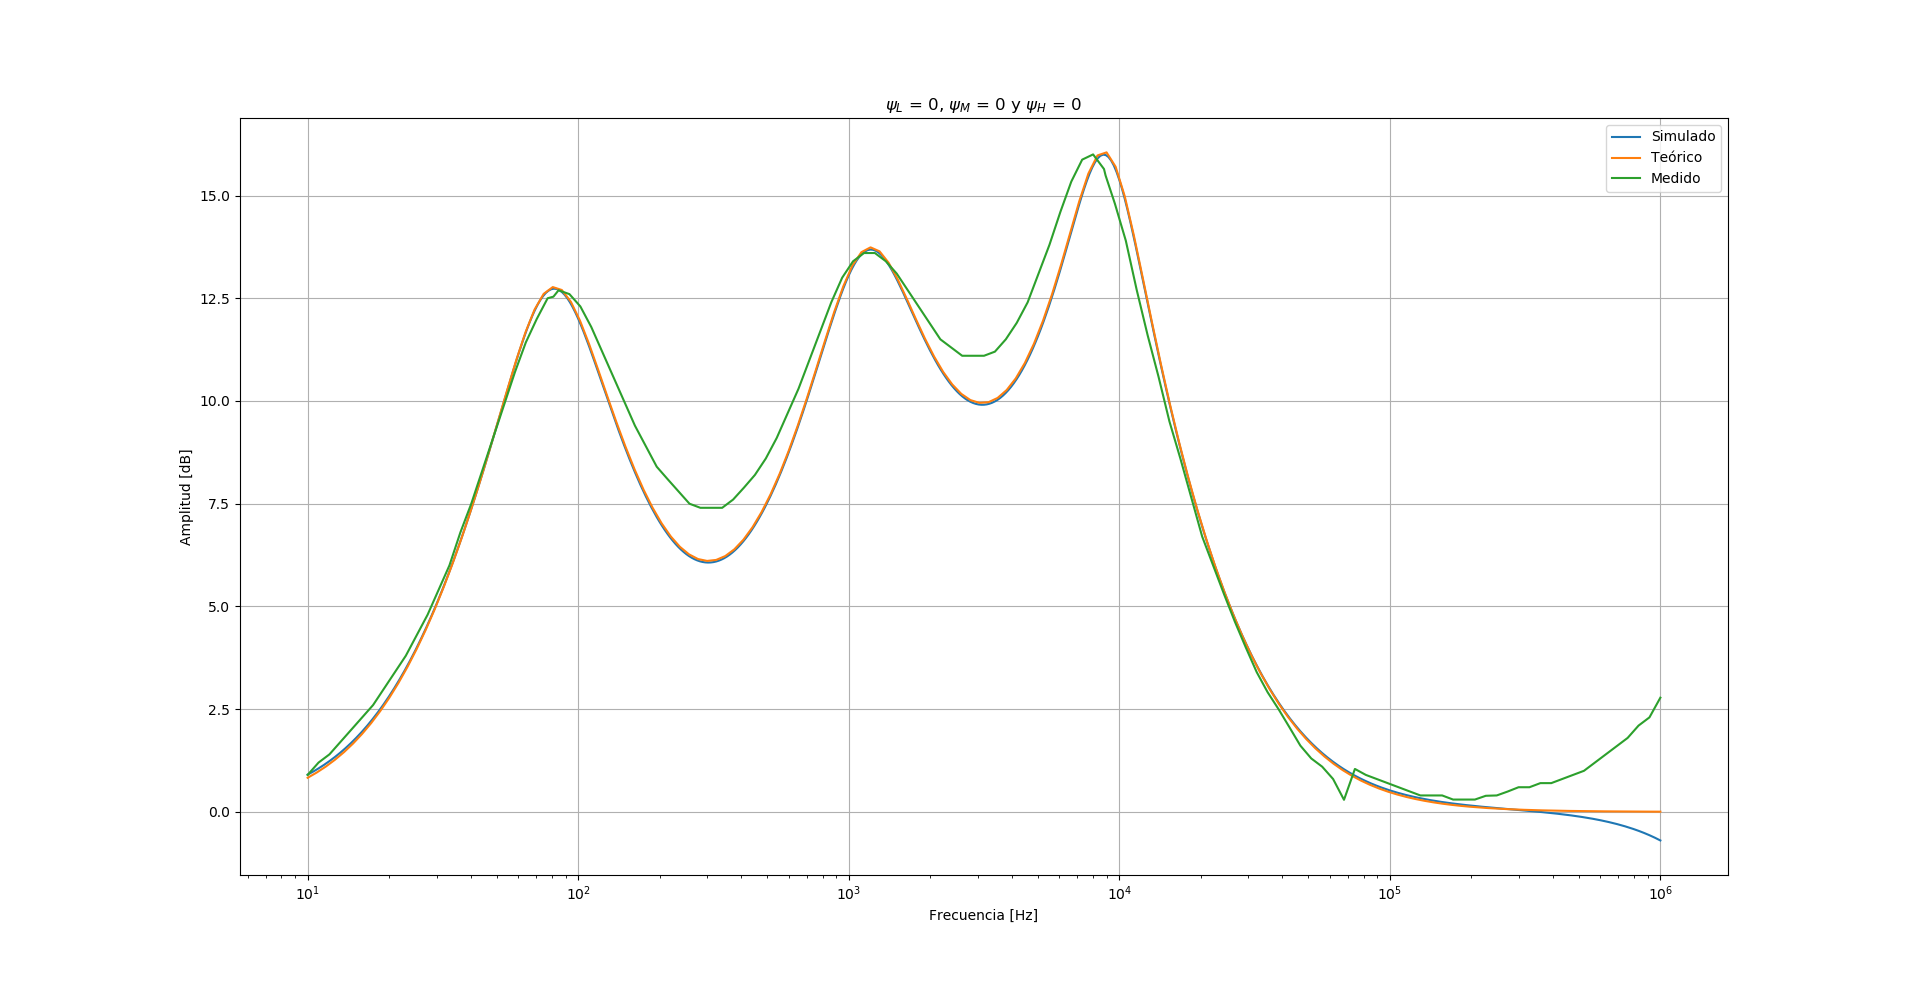
\includegraphics[width=0.9\textwidth]{Imagenes/CBodes-Mod-3.png}
	\caption{Diagrama de Bode en amplitud de la tercera medición.}
	\label{fig:CBodes-Mod-3}
\end{figure}
\begin{figure}[H]	
	\centering
	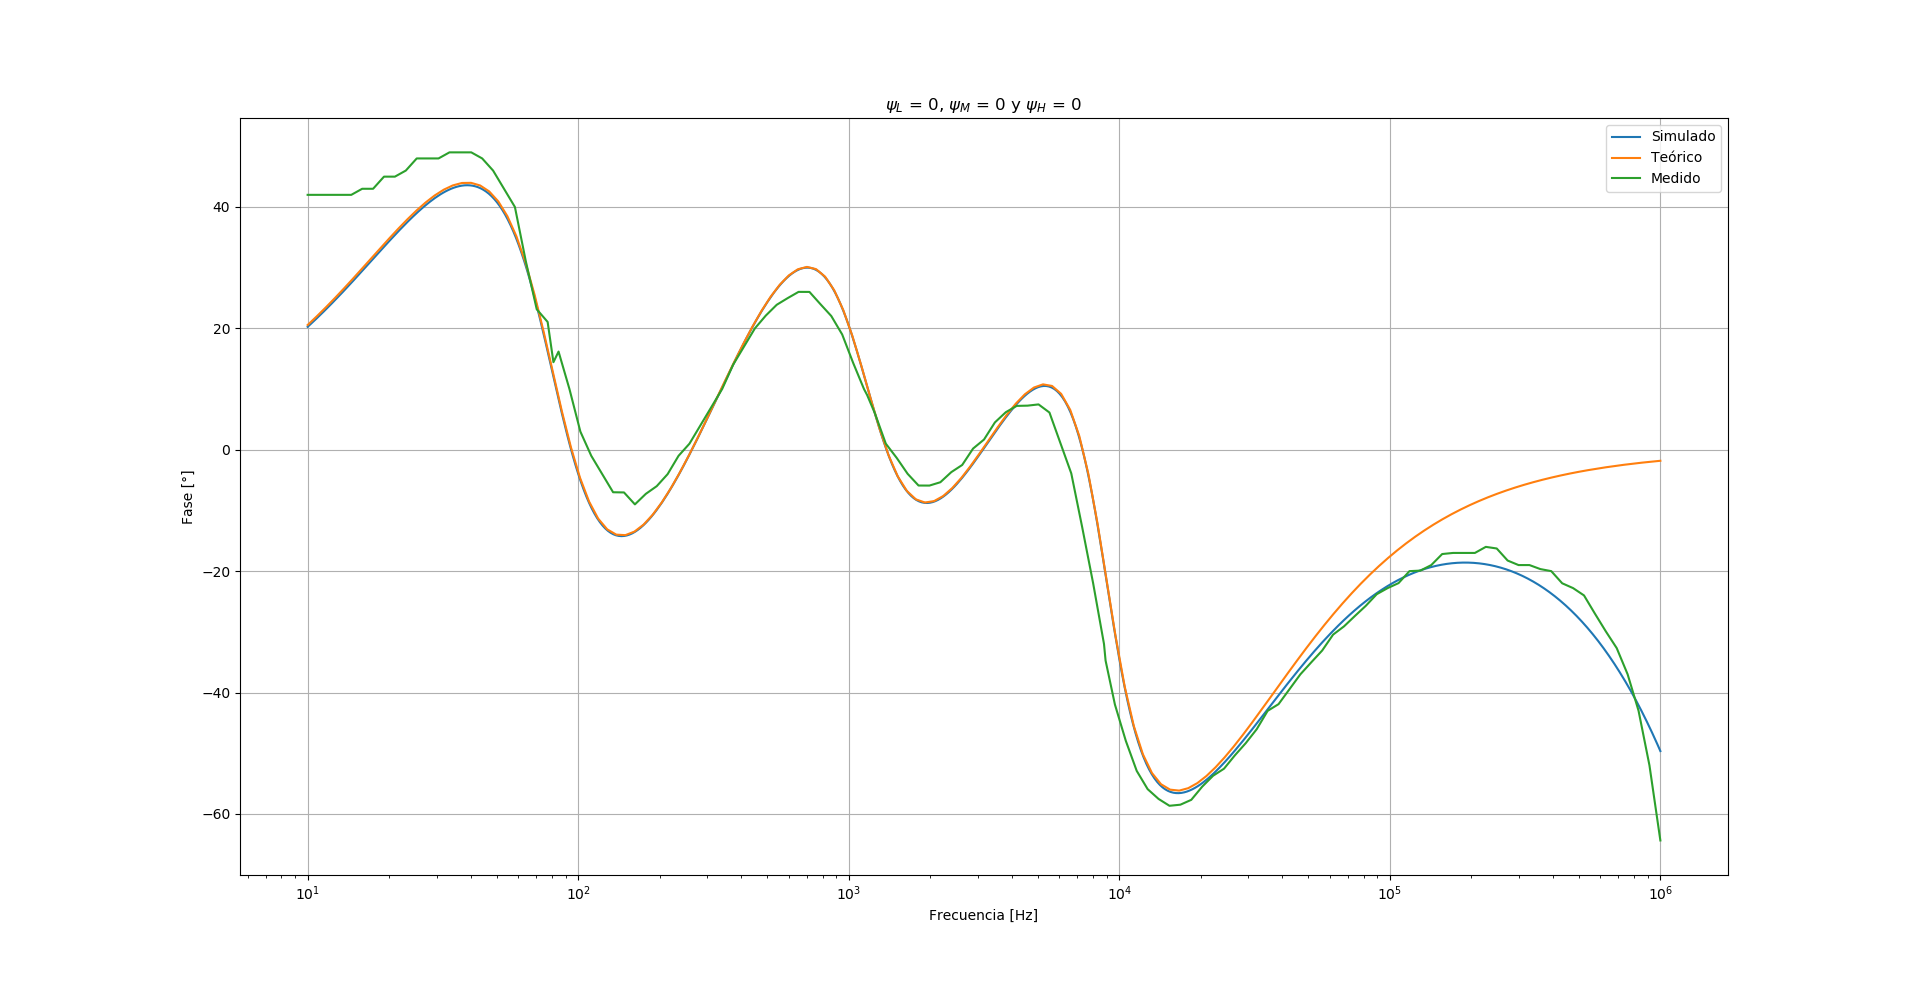
\includegraphics[width=0.9\textwidth]{Imagenes/CBodes-Ph-3.png}
	\caption{Diagrama de Bode en fase de la tercera medición.}
	\label{fig:CBodes-Ph-3}
\end{figure}
\begin{figure}[H]	
	\centering
	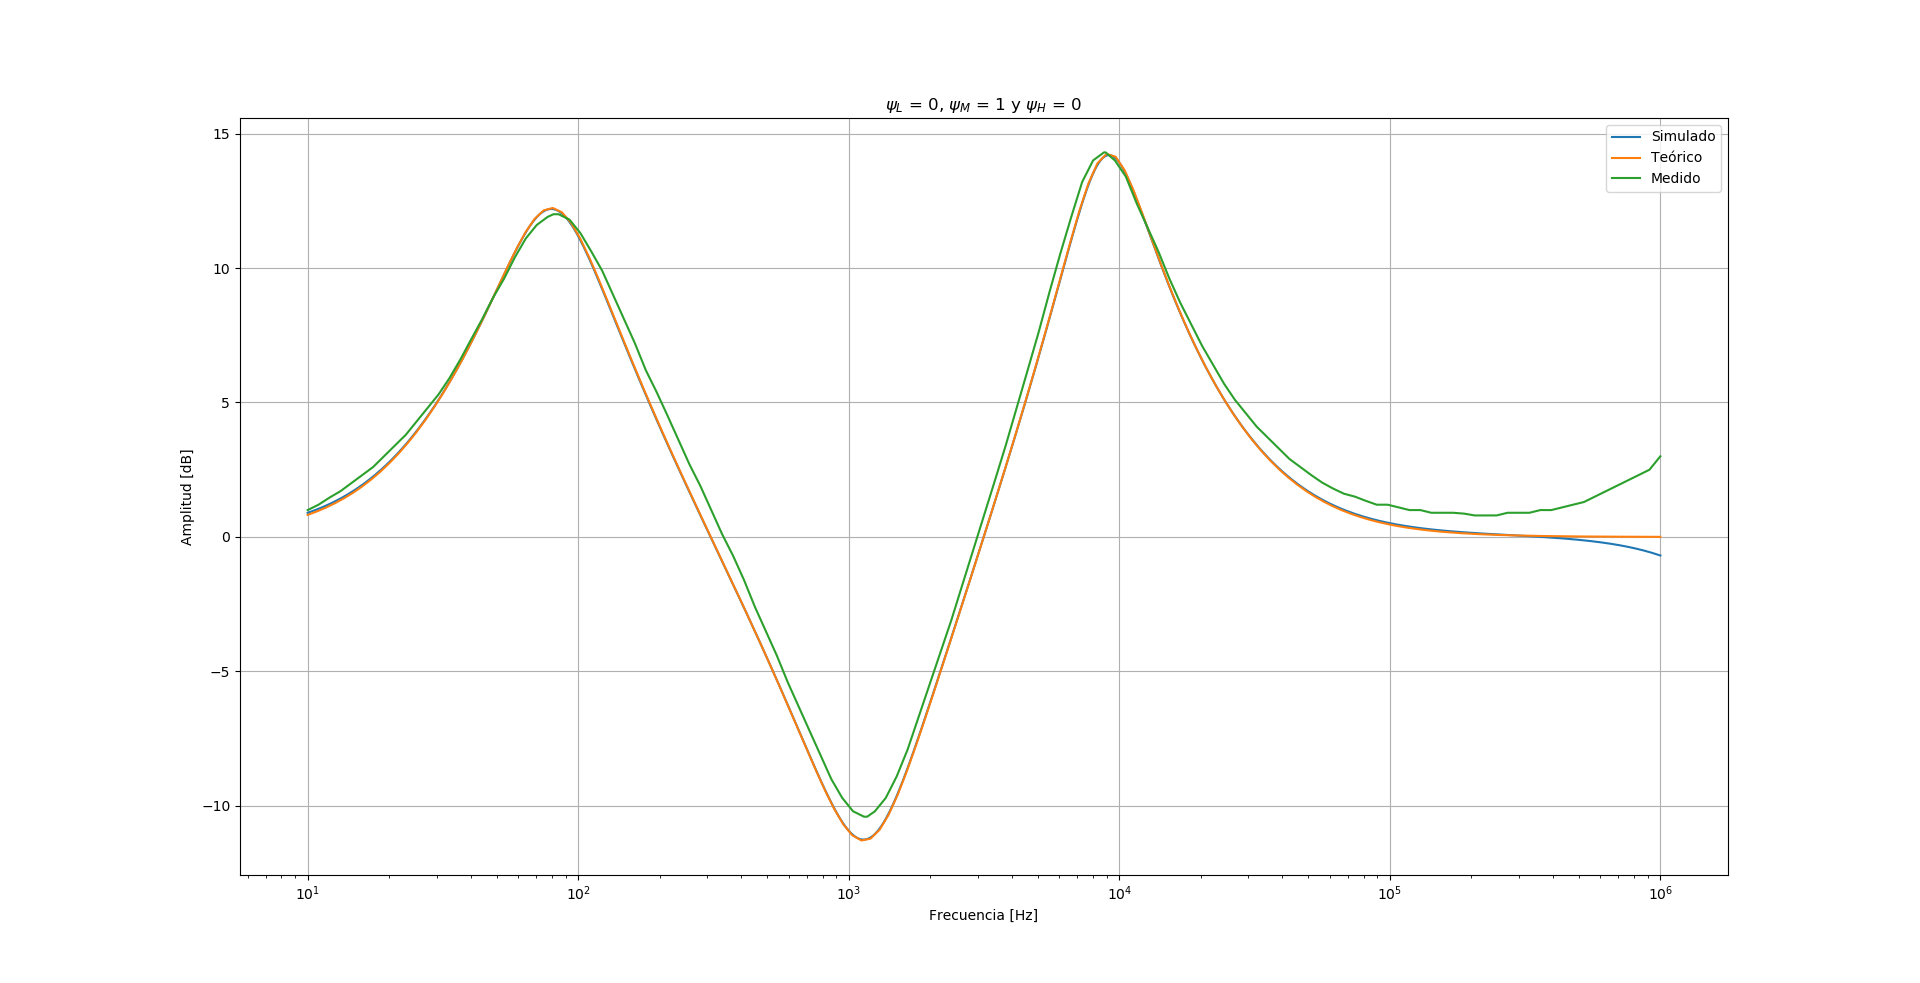
\includegraphics[width=0.9\textwidth]{Imagenes/CBodes-Mod-1.png}
	\caption{Diagrama de Bode en amplitud de la cuarta medición.}
	\label{fig:CBodes-Mod-4}
\end{figure}
\begin{figure}[H]	
	\centering
	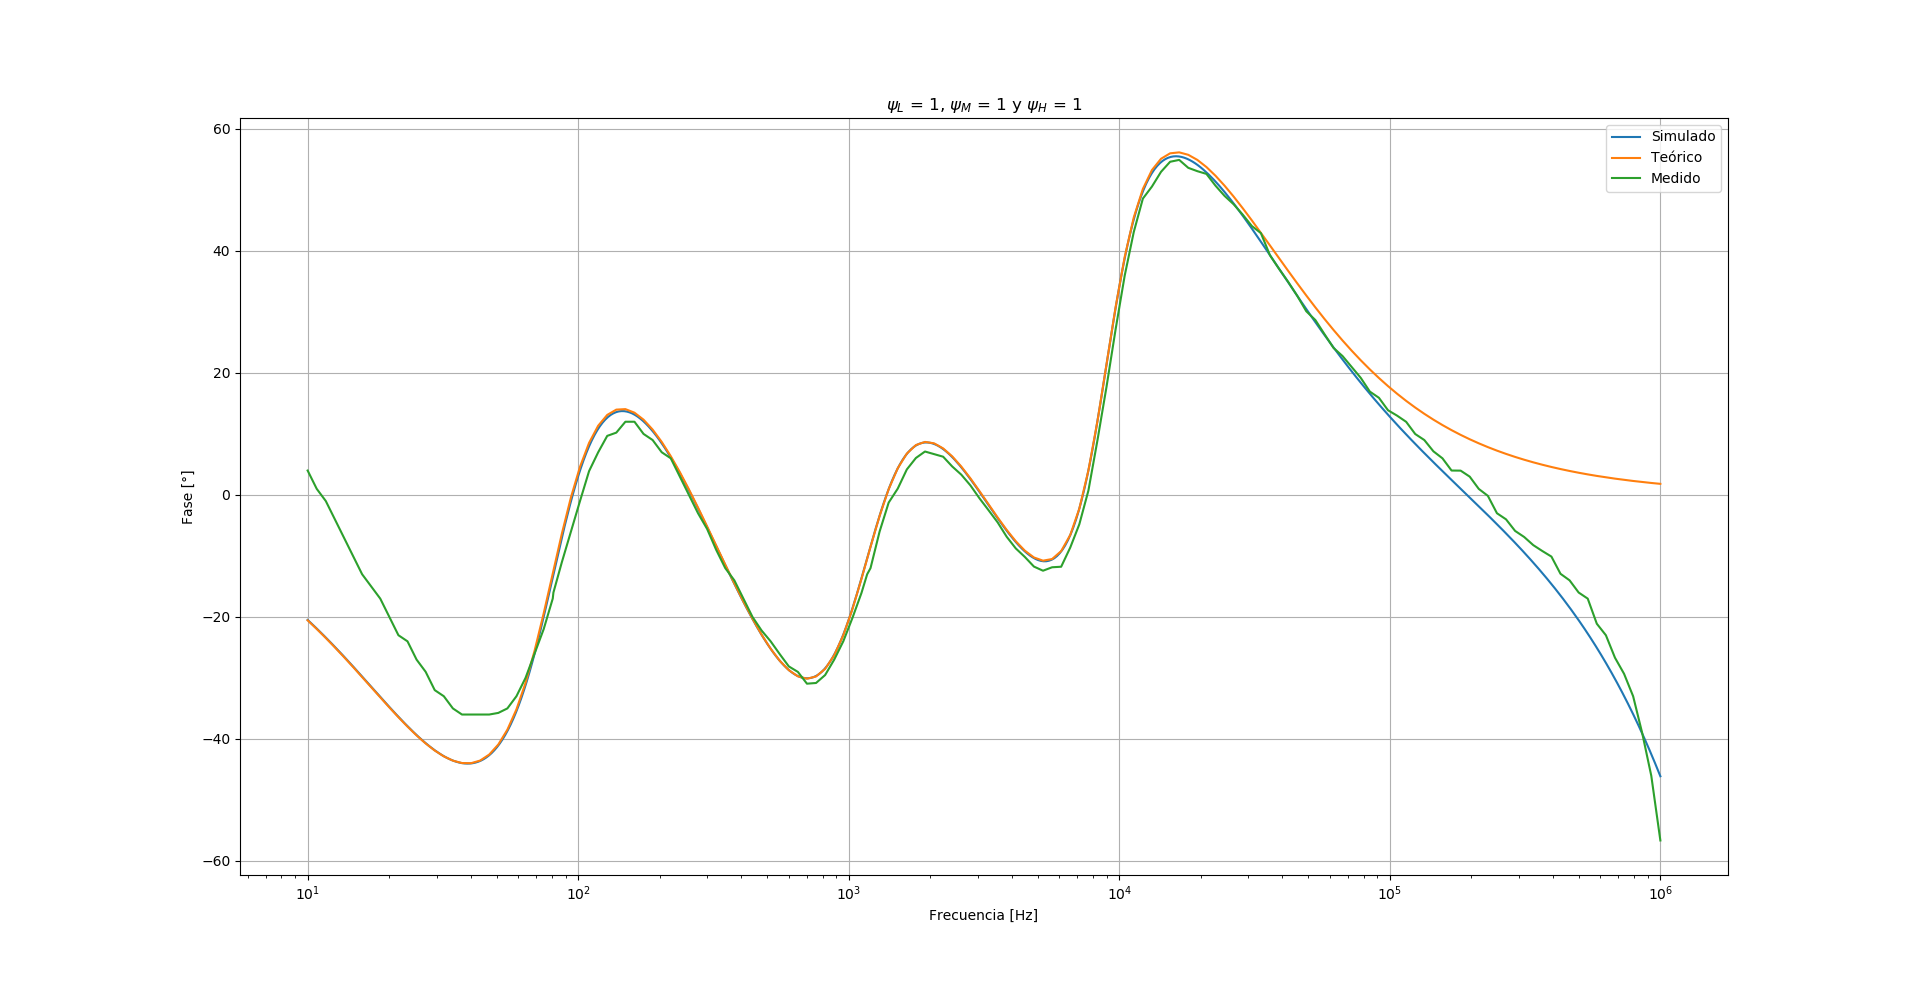
\includegraphics[width=0.9\textwidth]{Imagenes/CBodes-Ph-4.png}
	\caption{Diagrama de Bode en fase de la cuarta medición.}
	\label{fig:CBodes-Ph-4}
\end{figure}

Como se mostró en las Figuras (\ref{fig:MC-Mod}) y (\ref{fig:MC-Ph}), el hecho de poseer componentes con tolerancia baja, se termina de ver reflejado en las comparaciones previamente hechas. De estas, se puede concluir que, como los diagramas de Bode, tanto teóricos, como simulados y medidos, se acoplan adecuadamente, los diagramas de polos y ceros se corresponden. En otras palabras, los polos y ceros obtenidos en el circuito físico medido son similares a los obtenidos a través del modelo teórico. Finalmente, se destaca que en muy altas frecuencias, los diagramas no se corresponden en su totalidad. Este factor no es de interés y tampoco afecta el uso del circuito ya que estas diferencias se observan a partir de un rango de frecuencias mayor al audible, por lo tanto, el circuito no está destinado a trabajar en dicho intervalo.

%Por su parte, por lo visto en la Sección (\ref{sub:desarrollo}), la impedancia de entrada permanece prácticamente constante frente a cambios de $\psi$. De esta forma, se decidió presentar las comparaciones de dicha variable una sola vez, independientemente del valor de $\psi$.
%\begin{figure}[H]	
%	\centering
%	
\includegraphics[width=0.9\textwidth]{Imagenes/ZinCompMod.png}
%	\caption{Impedancia de entrada en modulo.}
%	\label{fig:ZinCompMod}
%\end{figure}
%\begin{figure}[H]	
%	\centering
%	
\includegraphics[width=0.9\textwidth]{Imagenes/ZinCompPh.png}
%	\caption{Impedancia de entrada en fase.}
%	\label{fig:ZinCompPh}
%\end{figure}

\subsubsection{Limitaciones}

Luego se destaca la limitación que presenta el circuito, en lo que a amplitud de tensión de entrada respecta. Como se destacó previamente, y debido a cuestiones de fabricación, entre cada etapa existe una pequeña diferencia en cuanto a amplificación (y atenuación) máxima se trata. Llegado a cierto punto, y bajo ciertas condiciones, el amplificador operacional satura la tensión de salida o se ve alterado por el efecto de Slew-Rate. De esta forma, se presentan a continuación las condiciones que hacen que cada etapa comience a presentar cambios en la salida.
\begin{figure}[H]	
	\centering
	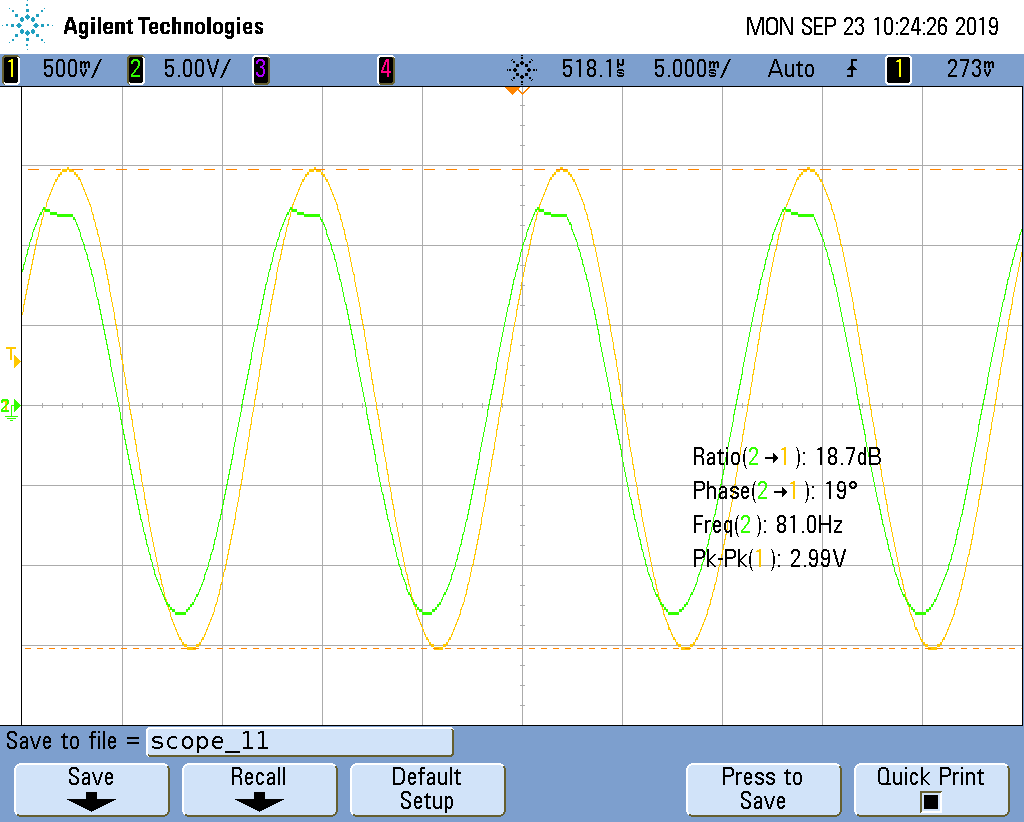
\includegraphics[width=0.6\textwidth, trim = {0 3.35cm 0 2cm},clip]{Imagenes/F81-3.png}
	\caption{Alteraciones de la salidas a frecuencias bajas.}
	\label{fig:F81-3}
\end{figure}
\begin{figure}[H]	
	\centering
	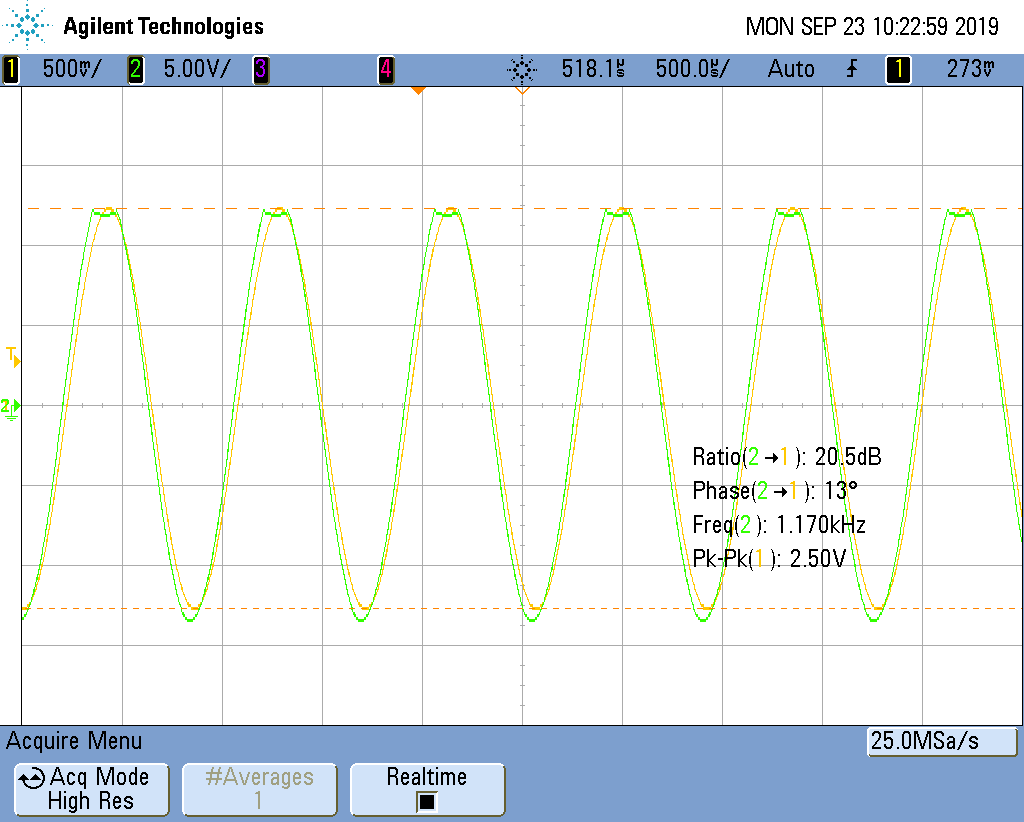
\includegraphics[width=0.6\textwidth, trim = {0 3.4cm 0 2cm},clip]{Imagenes/F1170-25.png}
	\caption{Alteraciones de la salidas a frecuencias medias.}
	\label{fig:F1170-25}
\end{figure}
\begin{figure}[H]	
	\centering
	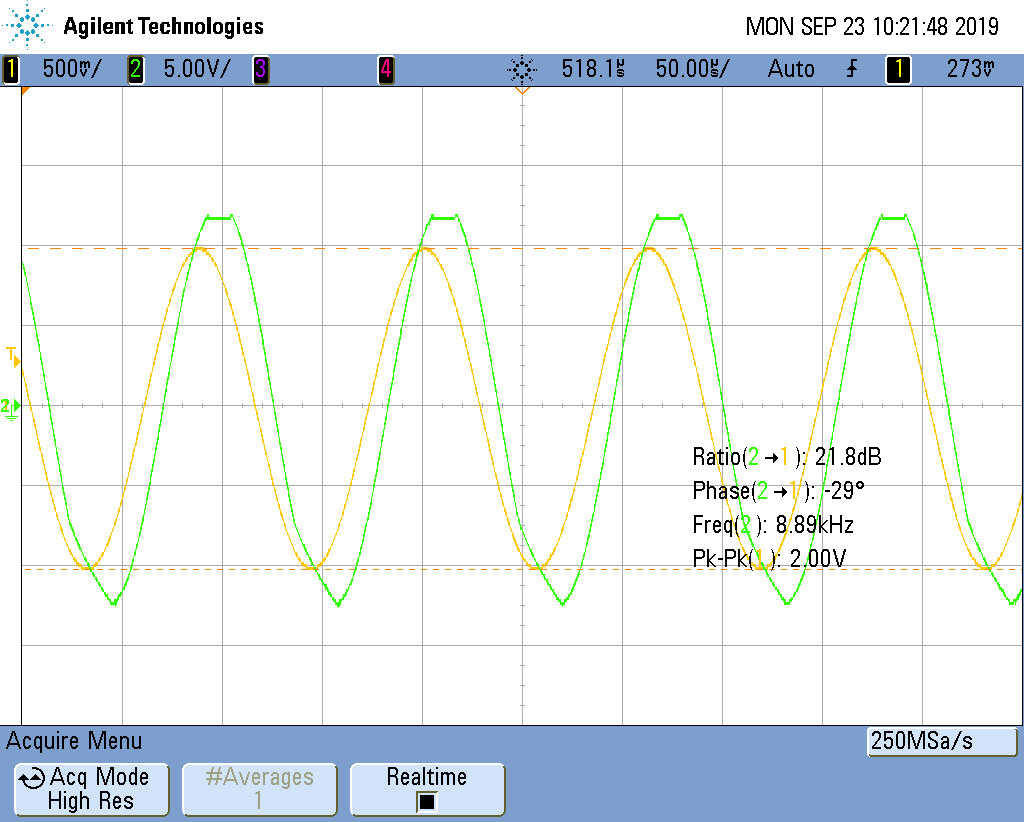
\includegraphics[width=0.6\textwidth, trim = {0 3.4cm 0 2cm},clip]{Imagenes/F8890-2.png}
	\caption{Alteraciones de la salidas a frecuencias altas.}
	\label{fig:F8890-2}
\end{figure}

Es por esta razón que se toma como límite una tensión de entrada máxima igual a $2 \ V$ (tensión pico a pico), ya que, a dicho valor ya comienza a observarse deformaciones en la salida para las frecuencias más altas, mientras que para las bajas y las medias se requieren tensiones de hasta $3 \ V$ y $2.5 \ V$ respectivamente. Esto se debe a que la etapa que posee mayor amplificación es aquella destinada a alterar las frecuencias altas.

\subsubsection{Aplicación}

Finalmente se realiza un breve comentario acerca su implementación. Se procedió a introducir a la entrada del circuito senoidales de una frecuencia dada, mientras que a la salida se colocaron parlantes para poder escuchar como la variación de cada instancia afecta la salida. Posteriormente se procedió realizar un experimento similar, pero esta vez colocando música a la entrada, más específicamente, ``Come as you are'' de Nirvana. Dicha experiencia fue grabada y se anexa en video junto con el informe. 